\section{Evaluation}
\label{sec:eval}
%
In this section, we study the performance characteristics of Algorithms~\ref{alg:inswrite} and \ref{alg:inswrite2}, NOrec, Hybrid NOrec, TLE and TL2.
Our experimental goals are: (G1) to study the performance impact of instrumentation on the fast-path and validation on the slow-path, 
%(G2) to understand how Algorithms~\ref{alg:inswrite} and \ref{alg:inswrite2} perform relative to the other algorithms,
(G2) to understand how HyTM algorithm design affects performance with Intel and IBM POWER8 HTMs, and 
(G3) to determine whether direct accesses can be used to obtain performance improvements on IBM POWER8 using the supported suspend/resume instruction to escape from a hardware transaction.

\vspace{1mm}\noindent\textbf{TM implementations.}
For TL2, we used the implementation published by its authors.
We implemented the other algorithms in C++.
Each hybrid TM algorithm first attempts to execute a transaction on the fast-path, and will continue to execute on the fast-path until the transaction has experienced 20 aborts, at which point it will fall back to the slow-path.
We implemented Algorithm~\ref{alg:inswrite} on POWER8 where each read of a sequence lock during a transactional read operation was enclosed within a pair of suspend/resume instructions to access them without 
incurring tracking set aborts (Algorithm~\ref{alg:inswrite}\textsuperscript{$\ast$}). We remark that this does not affect the opacity of the implementation. 
We also implemented the variant of Hybrid NOrec (Hybrid NOrec\textsuperscript{$\ast$}) in which the update to gsl is performed using a fetch-increment primitive between suspend/resume instructions, as is recommended in~\cite{hynorecriegel}.

In each algorithm, instead of placing a lock next to each address in memory, we allocated a global array of one million locks, and used a simple hash function to map each address to one of these locks.
This avoids the problem of having to change a program's memory layout to incorporate locks, and greatly reduces the amount of memory needed to store locks, at the cost of some possible false conflicts since many addresses map to each lock.
Note that the same approach was taken by the authors of TL2.

We chose \textit{not} to compile the TMs as separate libraries, since invoking library functions for each read and write can induce enormous overhead.
Instead, we compiled each TM directly into the code that uses it.
%Thus, any observed performance overheads are due to the algorithms, themselves.

\vspace{1mm}\noindent\textbf{Methodology.}
We used a simple unbalanced binary search tree (BST) microbenchmark as a vehicle to study the performance of our implementations.
The BST implements a dictionary, which contains a set of keys, each with an associated value.
For each TM algorithm %$A$ %\in \{$TL2, TLE, Algorithm~1, Algorithm~2, Hybrid NOrec$\}$,
and update rate $U \in \{40, 10, 0\}$, we run six timed \textit{trials} for several thread counts $n$.
Each trial proceeds in two phases: \textit{prefilling} and \textit{measuring}.
In the prefilling phase, $n$ concurrent threads perform 50\% \textit{Insert} and 50\% \textit{Delete} operations on keys drawn uniformly randomly from $[0, 10^K)$, where $K=5$ for our Intel machines and $K=4$ for our IBM POWER8 machine (since its HTM implementation is much more restrictive than Intel's, and there were too many aborts with the larger key range).
Prefilling continues until the size of the tree converges to a steady state (containing approximately $10^K/2$ keys).
Next, the trial enters the measuring phase, during which threads begin counting how many operations they perform.
In this phase, each thread performs $(U/2)$\% \textit{Insert}, $(U/2)$\% \textit{Delete} and $(100-U)$\% \textit{Search} operations, on keys/values drawn uniformly randomly from $[0,10^5)$, for ten seconds.
%% was it one second for old results?

Uniformly random updates to an unbalanced BST have been proven to yield trees of logarithmic height with high probability.
%Furthermore, updates and searches in an unbalanced BST are simple.
Thus, in this type of workload, almost all transactions succeed in hardware, and the slow-path is almost never used.
%there is no need. and have small read and write sets This workload is highly disjoint access parallel, and the height of the tree is relatively small, so most transactions succeed in hardware.
To study performance when transactions regularly run on slow-path, we introduced an operation called a \textit{RangeInc} that often fails in hardware and must run on the slow-path.
A \textit{RangeInc}$(low, hi)$ atomically increments the values 
associated with each key in the range $[low, hi]$ present in the tree.
Note that a \textit{RangeInc} is more likely to experience data 
conflicts and capacity aborts than typical BST updates, which only modify a single node.

We consider two types of workloads: (W1) all $n$ threads perform \textit{Insert}, \textit{Delete} and \textit{Search}, and (W2) $n-1$ threads perform \textit{Insert}, \textit{Delete} and \textit{Search} and one thread performs only \textit{RangeInc} operations.
%In W2, one can think of the thread $p$ that performs \textit{RangeInc} operations as a tunable knob that controls the fraction of time in the execution that the slow-path is being executed.
%Increasing the size of the range $[low, hi]$ passed to \textit{RangeInc} will cause $p$ to spend more time on the slow-path.




































\subsection{Experiments on IBM POWER8}

\vspace{1mm}\noindent\textbf{System.}
The experimental system (\textbf{POWER8}) is an IBM S822L with 2x 12-core 3.02GHz processor cards, 128GiB of RAM, running Ubuntu 16.04 LTS.
All code was compiled using G++ 5.3.1.
This is a dual socket machine, and each socket has two NUMA \emph{zones}.
It is expensive to access memory on a different NUMA zone, and even more expensive if the NUMA zone is on a different socket.
POWER8 uses the L2 cache for detecting tracking set aborts, and limits the size of a transaction's read- and write-set to 8KiB each~\cite{htm-survey}.
(This is in contrast to Intel which tracks conflicts on the entire L3 cache, and only limits a transaction's read-set to the L3 cache size, and its write-set to the L1 cache size.)

We pin one thread on each core within a NUMA zone before moving to the next zone.
We remark that unlike the thread pinning policy for Intel which saturated the first socket before moving to the next, this proved to be the best policy
for POWER8 which experiences severe negative scaling when threads are saturated on a single 8-way hardware multi-threaded core.
This is because all threads on a core share resources, including the L1 and L2 cache, a single branch execution pipeline, 
and only two load-store pipelines.


%As a way of validating correctness in each trial, each thread maintains a \textit{checksum}.
%Each time a thread inserts (resp., deletes) a key, it adds the key to (resp., subtracts from) its checksum.
%At the end of the trial, the sum of all thread checksums must be equal to the sum of keys in the tree.

\begin{figure}
    \centering
    \setlength\tabcolsep{0pt}
\begin{minipage}{1\linewidth}
    \centering
    \begin{tabular}{m{0.04\linewidth}m{0.48\linewidth}m{0.48\linewidth}}
        &
        \fcolorbox{black!50}{black!20}{\parbox{\dimexpr \linewidth-2\fboxsep-2\fboxrule}{\centering {0 threads perform \textit{RangeInc} (W1)}}} &
        \fcolorbox{black!50}{black!20}{\parbox{\dimexpr \linewidth-2\fboxsep-2\fboxrule}{\centering {1 thread performs \textit{RangeInc} (W2)}}}
        \\
        \rotatebox{90}{\large 0\% updates} &
        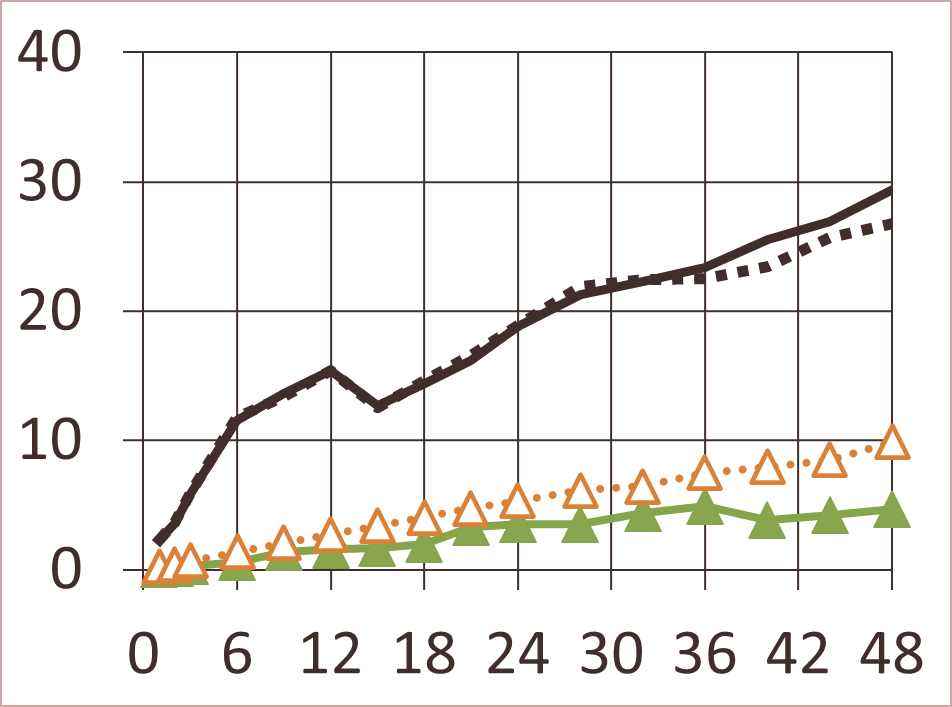
\includegraphics[width=\linewidth]{figures/2021jun16/power/dsbench3_2021_pivot_exp_0i0d10000k_nrq_0.png} &
        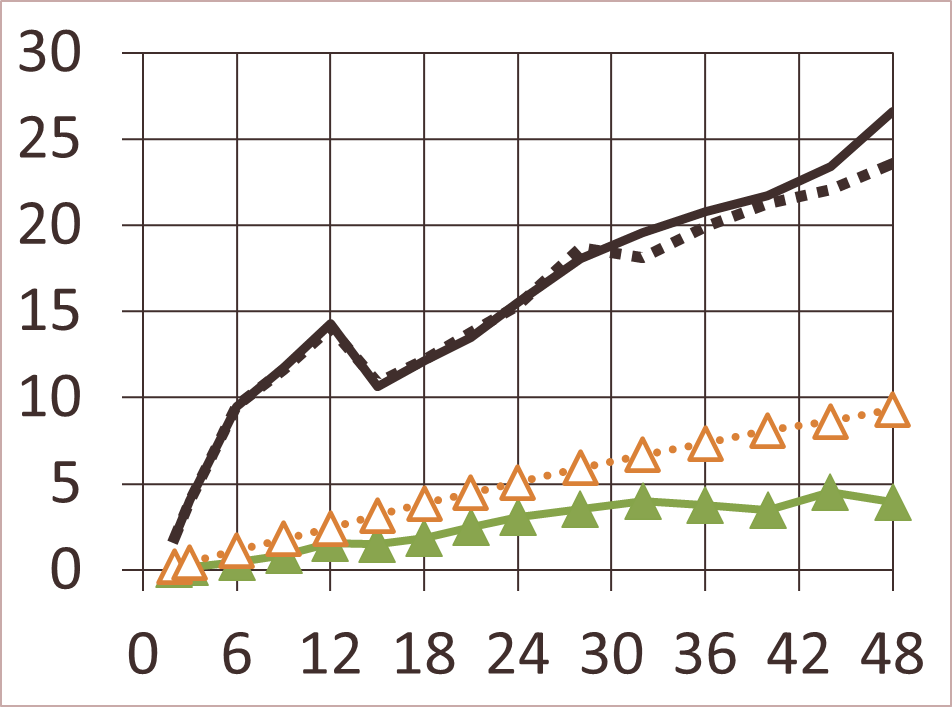
\includegraphics[width=\linewidth]{figures/2021jun16/power/dsbench3_2021_pivot_exp_0i0d10000k_nrq_1.png}
        \\
        \vspace{-8mm}\rotatebox{90}{\large 2\% updates} &
        \vspace{-8mm}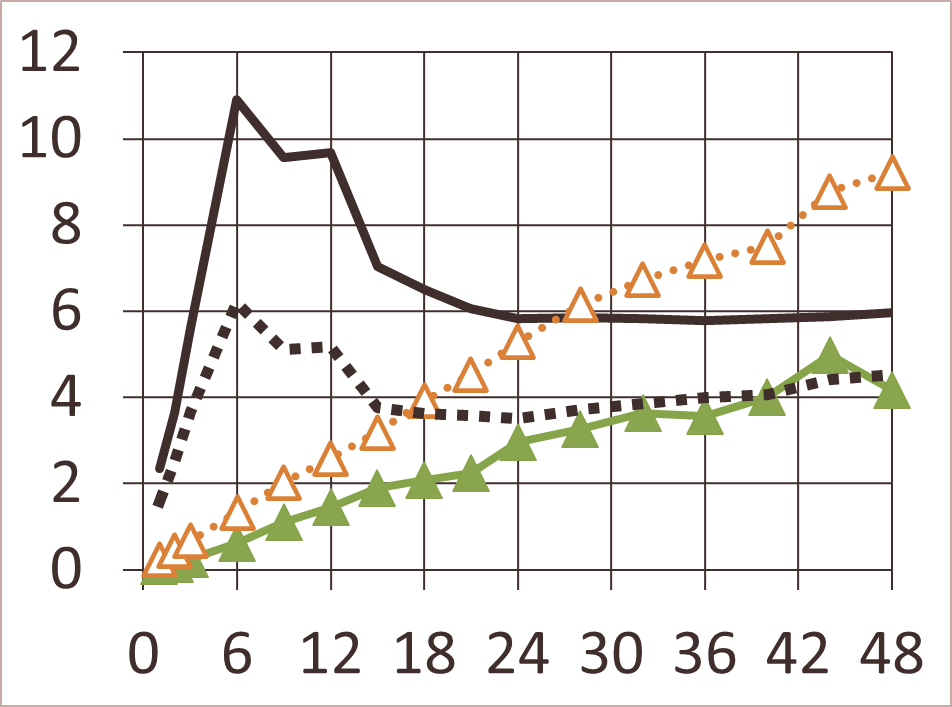
\includegraphics[width=\linewidth]{figures/2021jun16/power/dsbench3_2021_pivot_exp_1i1d10000k_nrq_0.png} &
        \vspace{-8mm}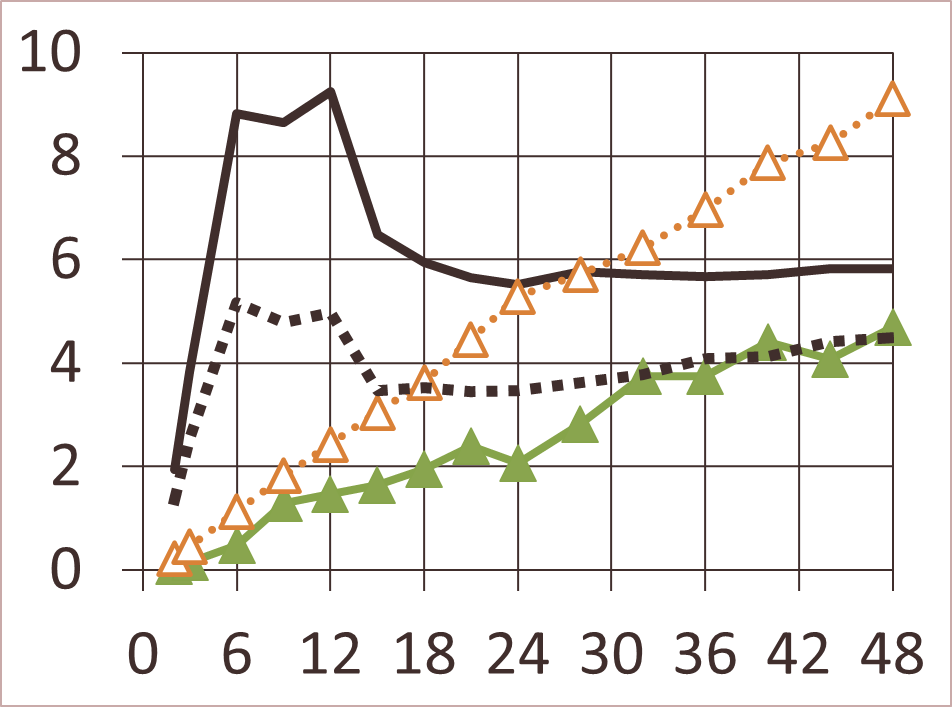
\includegraphics[width=\linewidth]{figures/2021jun16/power/dsbench3_2021_pivot_exp_1i1d10000k_nrq_1.png}
        \\
        \vspace{-8mm}\rotatebox{90}{\large 10\% updates} &
        \vspace{-8mm}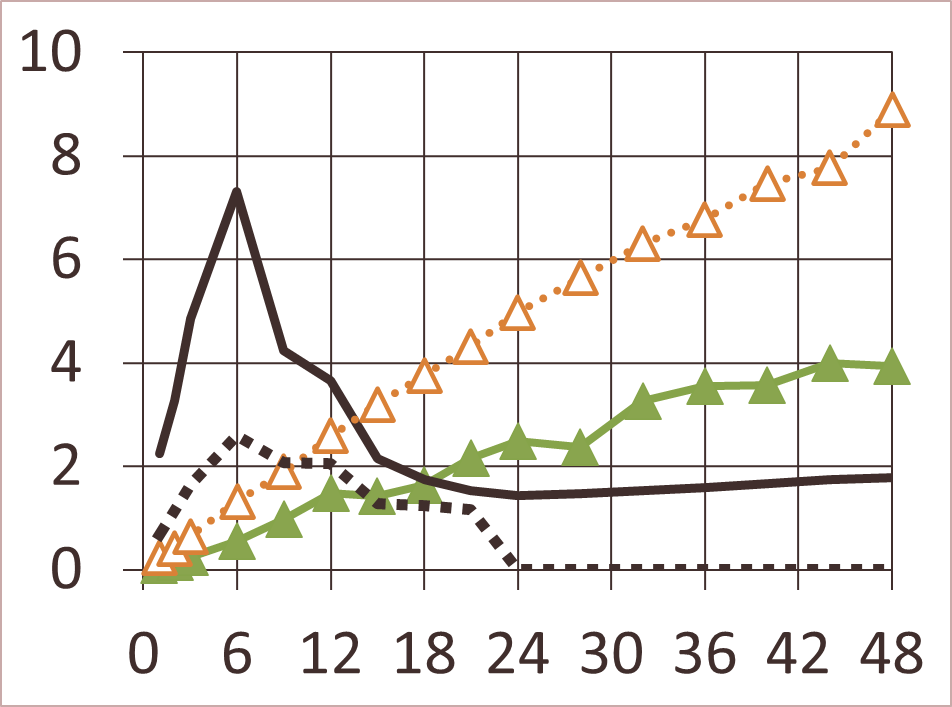
\includegraphics[width=\linewidth]{figures/2021jun16/power/dsbench3_2021_pivot_exp_5i5d10000k_nrq_0.png} &
        \vspace{-8mm}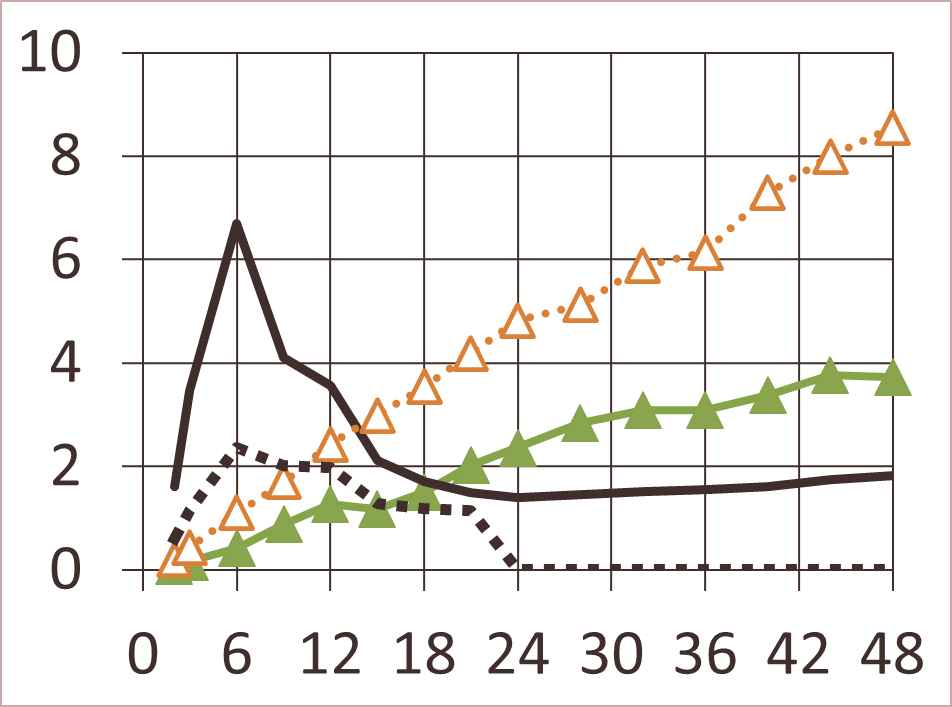
\includegraphics[width=\linewidth]{figures/2021jun16/power/dsbench3_2021_pivot_exp_5i5d10000k_nrq_1.png}
        \\
        \vspace{-8mm}\rotatebox{90}{\large 40\% updates} &
        \vspace{-8mm}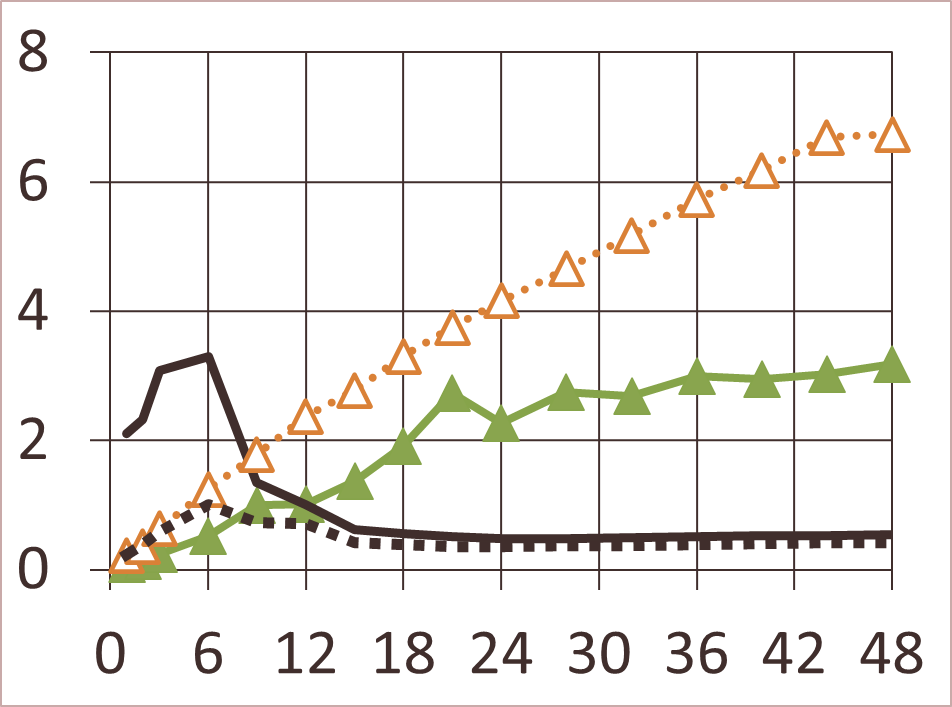
\includegraphics[width=\linewidth]{figures/2021jun16/power/dsbench3_2021_pivot_exp_20i20d10000k_nrq_0.png} &
        \vspace{-8mm}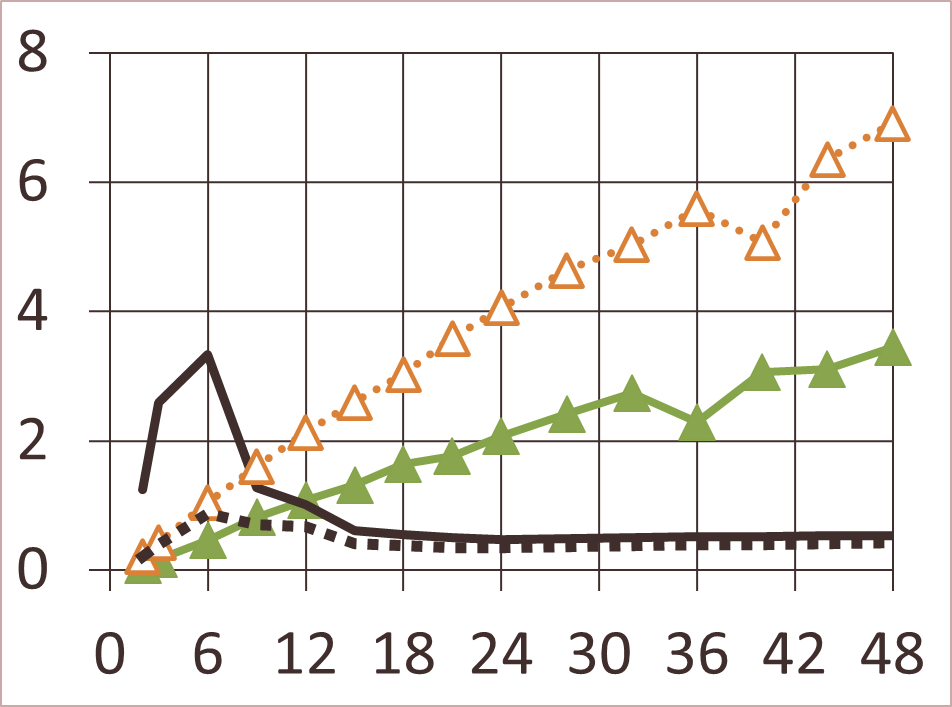
\includegraphics[width=\linewidth]{figures/2021jun16/power/dsbench3_2021_pivot_exp_20i20d10000k_nrq_1.png}
        \\
    \end{tabular}
\end{minipage}
    \vspace{-2mm}
	
\includegraphics[width=\linewidth]{figures/2021jun16/power/legend.png}
    \vspace{-2mm}
\caption{\textbf{POWER8} BST benchmark. x-axis: number of threads. y-axis: operations per $\mu$s.}
\label{fig-exp-power8}
\end{figure}

\vspace{1mm}\noindent\textbf{Discussion of results.}
See Figure~\ref{fig-exp-power8}.
%
Algorithm~\ref{alg:inswrite} performs poorly on POWER8: POWER8 transactions can only load 64 cache lines before they will abort~\cite{nguyen-thesis}. 
Transactions read locks and tree nodes, which are in different cache lines: together, they often exceed 64 cache lines loaded in a tree operation, 
so most transactions cannot succeed in hardware. Consequently, on POWER8, 
it is incredibly important either to have minimal instrumentation in transactions, or for metadata to be located in the 
same cache lines as program data. Of course, the latter is not possible for HyTMs, which do not have control over the layout of program data.
Consequently, Algorithm~\ref{alg:inswrite2} outperforms Algorithm~\ref{alg:inswrite} in POWER8 quite easily by avoiding the per-read instrumentation. 

Algorithm~\ref{alg:inswrite} is improved slightly by the expensive (on POWER8) suspend/resume on sequence locks during transactional reads, but it still performs relatively poorly. 
To make suspend/resume a practical tool, one could imagine attempting to 
collect several metadata accesses and perform them together to amortize the cost of a suspend/resume pair. For instance, 
in Algorithm~\ref{alg:inswrite}, one might try to update the locks for all of the transactional writes at once, when the transaction commits. 
Typically one would accomplish this by logging all writes so that a process can remember which addresses it must lock at commit time. 
However, logging the writes inside the transaction would be at least as costly as just performing them.

Observe that Hybrid NOrec does far worse with updates in POWER8 than on the Intel machine.
This is due to the fact that fetch-increment on a single location experiences severe negative scaling on the POWER8 processor: e.g., in one second, a single
thread can perform 37 fetch-add operations while 6 threads perform a total of 9 million and 24 threads perform only 4 million fetch-add operations.
In contrast, the Intel machine performs 32 million operations with 6 threads and 45 million with 24 threads. This is likely because this Intel processor provides 
fetch-add instructions while it must be emulated on the POWER8 processor.

In Hybrid NOrec\textsuperscript{$\ast$}, the non-speculative increment of gsl actually makes performance worse. Recall that in Hybrid NOrec, 
if a fast-path transaction $T_1$ increments gsl, and then a software transaction $T_2$ reads gsl (as part of validation) before $T_1$ commits, then $T_1$ will abort, 
and $T_2$ will not see $T_1$'s change to gsl. 
So, $T_2$ will have a higher chance of avoiding incremental validation (and, hence, will likely take less time to run, and have a smaller contention window).
However, in Hybrid NOrec\textsuperscript{$\ast$}, once $T_1$ increments gsl, $T_2$ will see the change to gsl, regardless of whether $T_1$ commits or aborts. Thus, 
$T_2$ will be forced to perform incremental validation. In our experiments, we observed that a much larger number of transactions ran on 
the fallback path in Hybrid NOrec\textsuperscript{$\ast$} than in Hybrid NOrec (often several orders of magnitude more).


%\subsection{Experiments on Intel Xeon v3}
%
%\begin{figure}
%    \centering
%    \setlength\tabcolsep{0pt}
%\begin{minipage}{1\linewidth}
%    \centering
%    \begin{tabular}{m{0.03\linewidth}m{0.485\linewidth}m{0.485\linewidth}}
%        &
%        \fcolorbox{black!50}{black!20}{\parbox{\dimexpr \linewidth-2\fboxsep-2\fboxrule}{\centering {0 threads perform \textit{RangeInc} (W1)}}} &
%        \fcolorbox{black!50}{black!20}{\parbox{\dimexpr \linewidth-2\fboxsep-2\fboxrule}{\centering {1 thread performs \textit{RangeInc} (W2)}}}
%        \\
%        \rotatebox{90}{\large 0\% updates} &
%        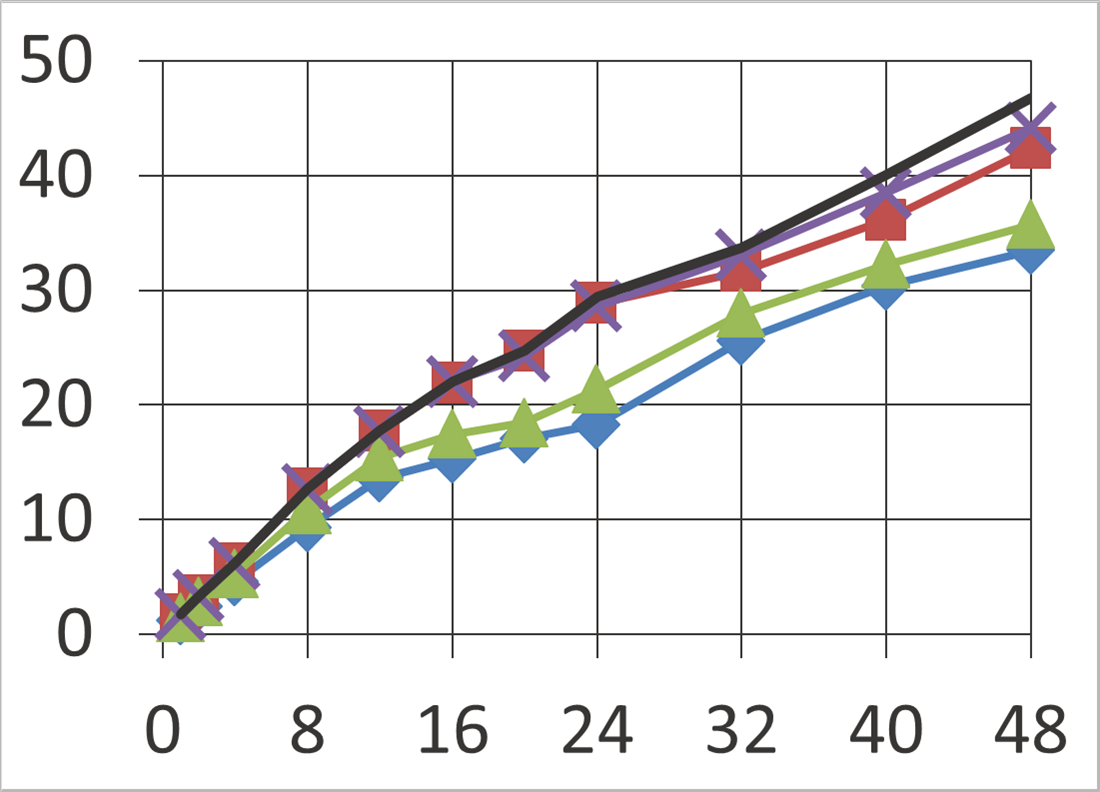
\includegraphics[width=\linewidth]{figures/graphs/0i0d100000k-nrq0.png} &
%        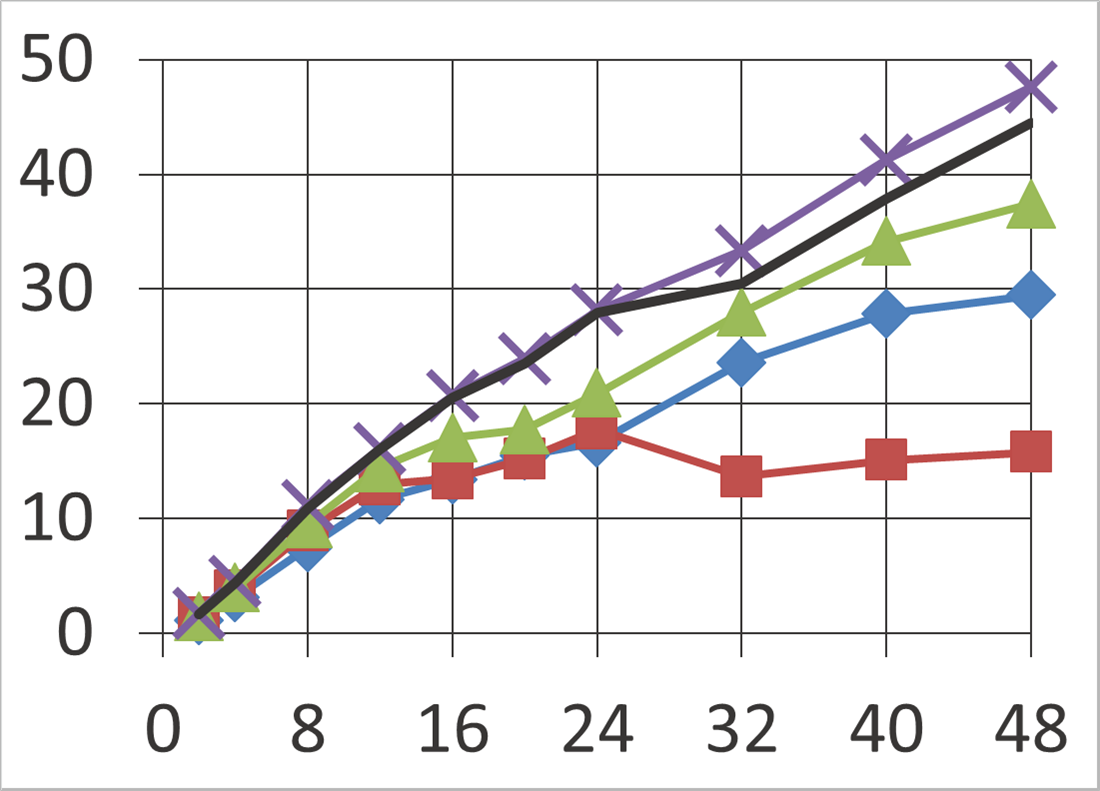
\includegraphics[width=\linewidth]{figures/graphs/0i0d100000k-nrq1.png}
%        \\
%        \vspace{-8mm}\rotatebox{90}{\large 10\% updates} &
%        \vspace{-8mm}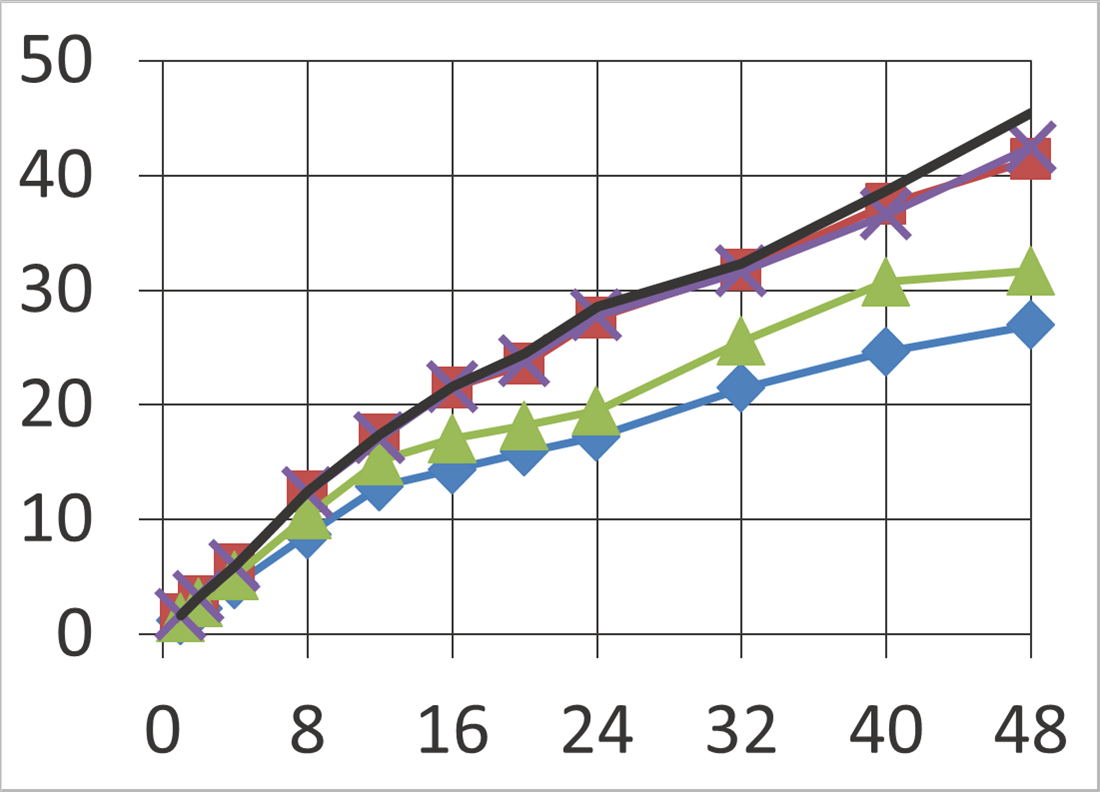
\includegraphics[width=\linewidth]{figures/graphs/5i5d100000k-nrq0.png} &
%        \vspace{-8mm}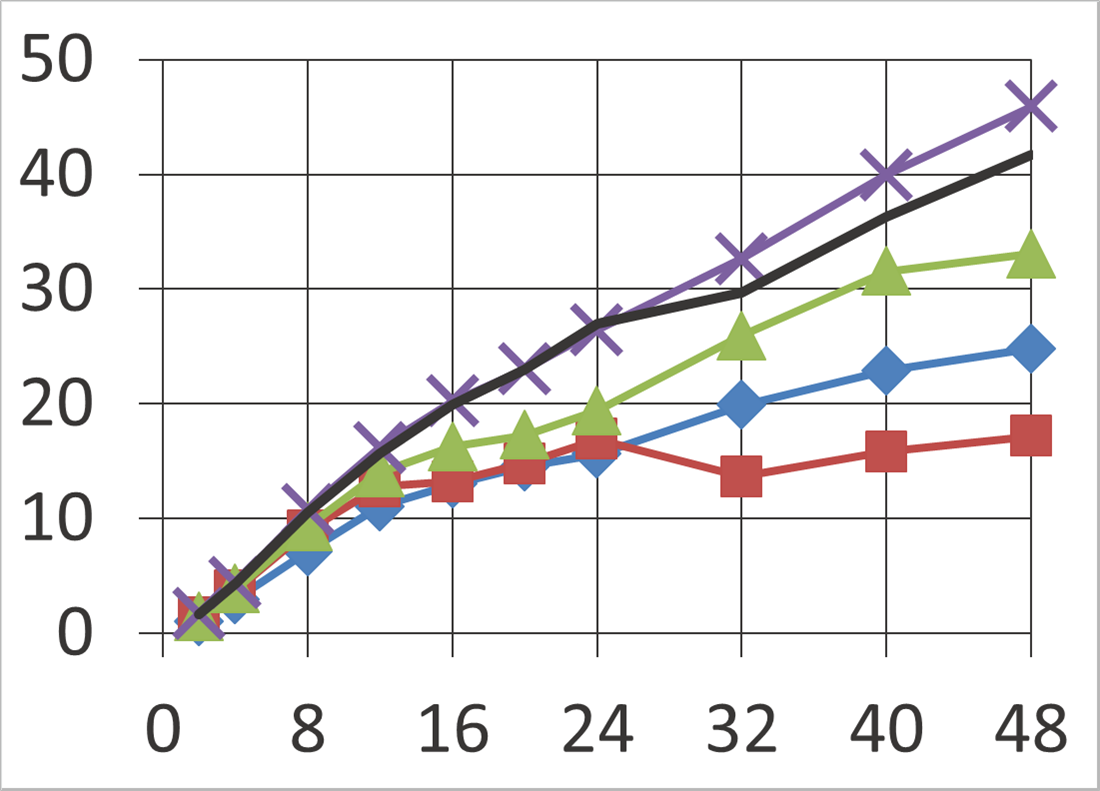
\includegraphics[width=\linewidth]{figures/graphs/5i5d100000k-nrq1.png}
%        \\
%        \vspace{-8mm}\rotatebox{90}{\large 40\% updates} &
%        \vspace{-8mm}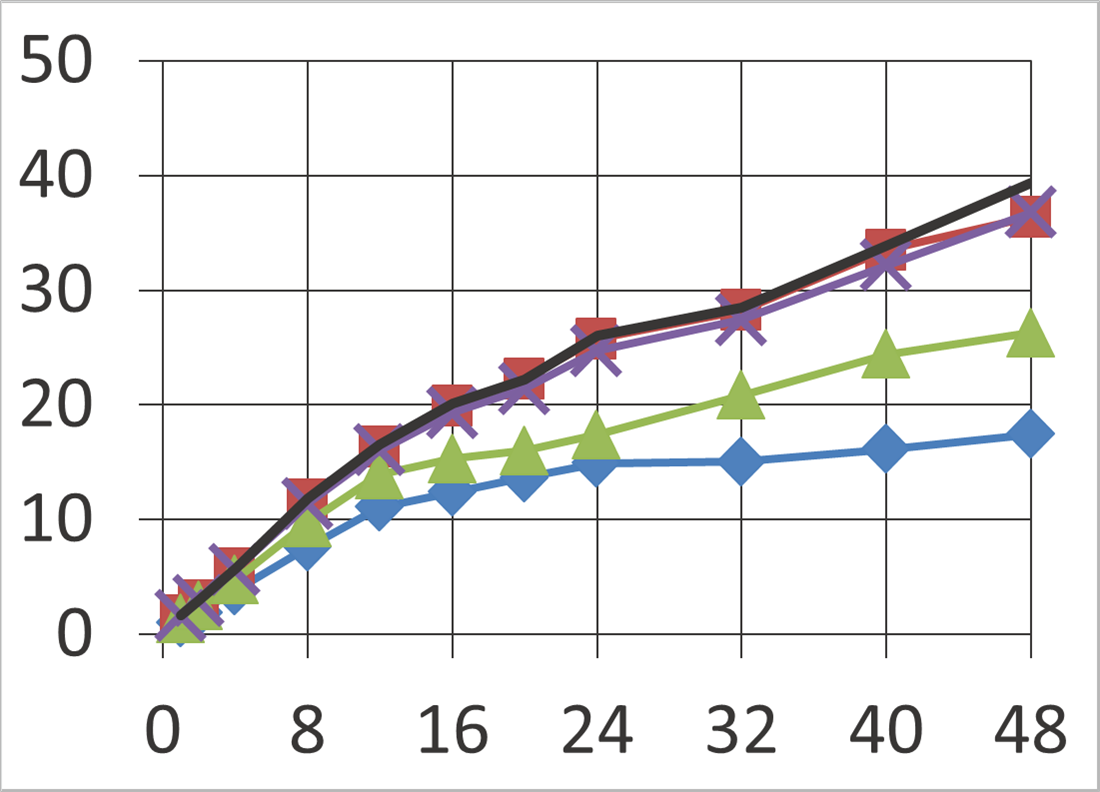
\includegraphics[width=\linewidth]{figures/graphs/20i20d100000k-nrq0.png} &
%        \vspace{-8mm}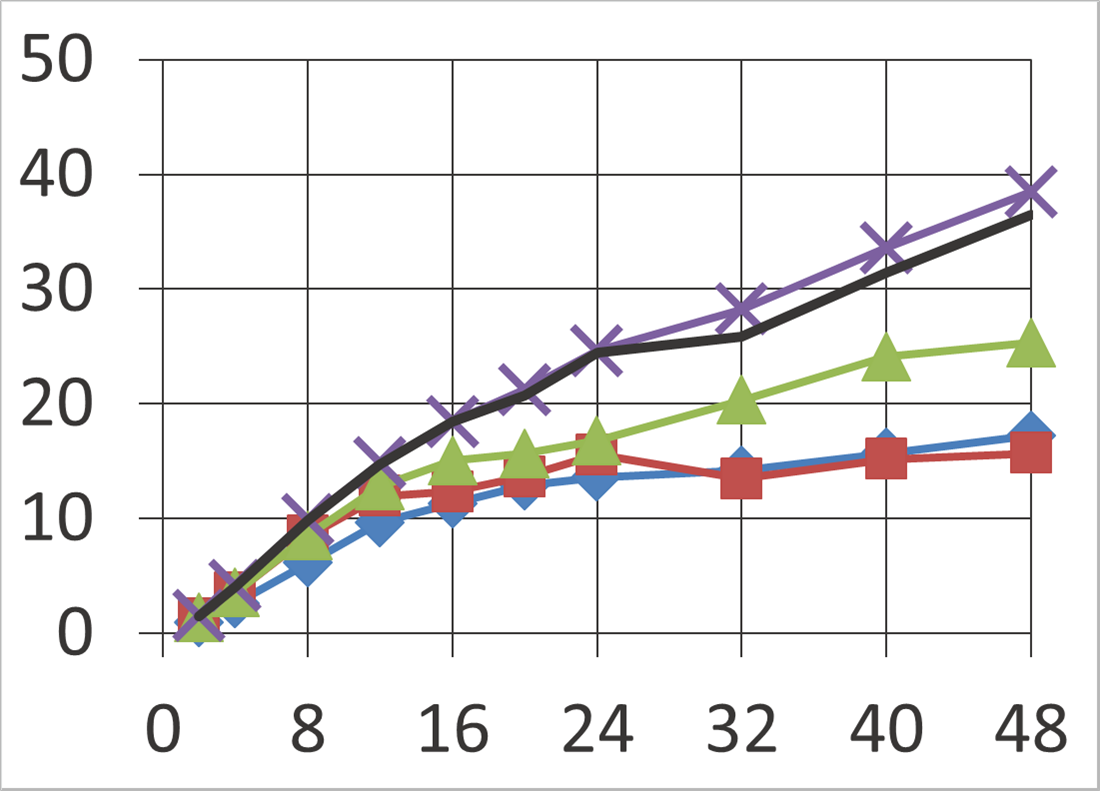
\includegraphics[width=\linewidth]{figures/graphs/20i20d100000k-nrq1.png}
%        \\
%    \end{tabular}
%\end{minipage}
%    \vspace{-2mm}
%	
\includegraphics[width=\linewidth]{figures/graphs/power8/dsbench3_legend_power.png}
%    \vspace{-2mm}
%\caption{\textbf{XeonV3} BST benchmark. x-axis: number of threads. y-axis: operations per $\mu$s.}
%\label{fig-exp-xeonv3}
%\end{figure}
%
%
%\vspace{1mm}\noindent\textbf{System.}
%The experimental system (\textbf{XeonV3}) is a 2-socket Intel Xeon E7-4830 v3 with 12 cores per socket and 2 hyperthreads (HTs) per core, for a total of 48 threads.
%Each core has a private 32KiB L1 cache and 256KiB L2 cache (shared between HTs on a core).
%All cores on a socket share a 30MiB L3 cache.
%This system has a non-uniform memory architecture (NUMA) in which threads have significantly different access costs to different parts of memory depending on which processor they are currently executing on.
%The machine has 128
% of RAM, and runs Ubuntu 14.04 LTS.
%All code was compiled with the GNU C++ compiler (G++) 4.8.4 with build target x86\_64-linux-gnu and compilation options \texttt{-std=c++0x -O3 -mx32}.
%
%We pin threads so that the first socket is saturated before we place any threads on the second socket.
%Thus, thread counts 1-24 run on a single socket.
%Furthermore, hyperthreading is engaged on the first socket for thread counts 13-24, and on the second socket for thread counts 37-48.
%Consequently, our graphs clearly show the effects of NUMA and hyperthreading.
%%Thread support was provided by the POSIX Threads library.
%%We used the default glibc allocator.
%
%
%\vspace{1mm}\noindent\textbf{Results.}
%See Figure~\ref{fig-exp-xeonv3}.
%We first discuss the 0\% updates graph for workload type W1.
%In this graph, essentially all operations committed in hardware.
%In fact, in each trial, a small fraction of 1\% of operations ran on the slow-path.
%Thus, any performance differences shown in the graph are essentially differences in the performance of the algorithms' respective fast-paths (with the exception of TL2).
%Algorithm~\ref{alg:inswrite}, which has instrumentation in its fast-path read operations, has significantly lower performance than Algorithm~\ref{alg:inswrite2}, which does not.
%Since this is a read-only workload, this instrumentation is responsible for the performance difference.
%
%In the W1 workloads, TLE, Algorithm~\ref{alg:inswrite2} and Hybrid NOrec perform similarly (with a small performance advantage for Hybrid NOrec at high thread counts).
%This is because the fast-paths for these three algorithms have similar amounts of instrumentation: there is no instrumentation for reads or writes, 
%and the transaction itself incurs one or two metadata accesses.
%In contrast, in the W2 workloads, TLE performs quite poorly, compared to the HyTM algorithms.
%In these workloads, transactions must periodically run on the slow-path, and in TLE, 
%this entails acquiring a global lock that restricts progress for all other threads.
%At high thread counts this significantly impacts performance.
%Its performance decreases as the sizes of the ranges passed to \textit{RangeInc} increase.
%Its performance is also negatively impacted by NUMA effects at thread counts higher than 24.
%(This is because, when a thread $p$ reads the lock and incurs a cache miss, 
%if the lock was last held by another thread on the same socket, 
%then $p$ can fill the cache miss by loading it from the shared L3 cache.
%However, if the lock was last held by a thread on a different socket, 
%then $p$ must read the lock state from main memory, which is significantly more expensive.)
%On the other hand, in each graph in the W2 workloads, the performance of each HyTM (and TL2) is similar to its performance in the corresponding W1 workload graph.
%For Algorithm~\ref{alg:inswrite} (and TL2), this is because of progressiveness.
%Although Algorithm~\ref{alg:inswrite2} is not truly progressive, fast-path transactions will abort only if they are concurrent with the commit procedure of a slow-path transaction.
%In \textit{RangeInc} operations, there is a long read-only prefix (which is exceptionally long because of Algorithm~\ref{alg:inswrite2}'s quadratic validation) followed by a relatively small set of writes.
%Thus, \textit{RangeInc} operations have relatively little impact on the fast-path.
%The explanation is similar for Hybrid NOrec (except that it performs less validation than Algorithm~\ref{alg:inswrite2}).
%
%Observe that the performance of Hybrid NOrec decreases slightly, relative to Algorithm~\ref{alg:inswrite2}, after 24 threads.
%Recall that, in Hybrid NOrec, the global sequence number is a single point of contention on the fast-path.
%(In Algorithm~\ref{alg:inswrite2}, the global lock is only modified by slow-path transactions, so fast-path transactions do not have a single point of contention.)
%We believe this is due to NUMA effects, similar to those described in~\cite{BKLL16}.
%Specifically, whenever a threads on the first socket performs a fast-path transaction that commits and modifies the global lock, it causes cache invalidations for all other threads.
%Threads on socket two must then load the lock state from main memory, which takes much longer than loading it from the shared L3 cache.
%This lengthens the transaction's window of contention, making it more likely to abort.
%(In the 0\% updates graph in the W2 workload, we still see this effect, because there is a thread performing \textit{RangeInc} operations.)
%%% IF THIS DISCREPANCY IS DUE TO NUMA EFFECTS HURTING UPDATES, WHY DOES THE GAP BETWEEN ALGORITHMS DECREASE AS THE NUMBER OF UPDATES INCREASES?
%% here's a subtle hypothesis. there are two different numa effects competing to be the dominating performance factor. one is the effect i just described above. the other is the negative performance impact of tree updates on traversals. this is something we saw in the oracle spaa paper when looking at tree updates in htm. i expect that the strength of the negative numa effects on tree traversals with increased updates is greater than the strength of the negative numa effects of esl and gsl updates. since the negative effects on tree traversals impact both algorithms, it makes the difference in performance less significant, masking the other numa effect.

\subsection{Experiments on Intel Xeon Scalable}

\vspace{1mm}\noindent\textbf{Experimental system.}
The experimental system (\textbf{XeonGold}) is a 4-socket Intel Xeon Scalable Series Platinum 8160 with 24 cores per socket and 2 hyperthreads (HTs) per core, for a total of 192 threads.
Each core has a private 32KiB L1 cache and 1MiB L2 cache (shared between HTs on a core).
All cores on a socket share a 33MiB L3 cache.
This system has a non-uniform memory architecture (NUMA) in which threads have significantly different access costs to different parts of memory depending on which processor they are currently executing on.
The machine has 392GiB of RAM, and runs Ubuntu 18.04 LTS.
All code was compiled with the GNU C++ compiler (G++) 10.1 with maximum optimization.

We pin threads so that the first socket is saturated before we place any threads on the second socket.
Thus, thread counts 1-48 run on a single socket.
Hyperthreading is engaged on the first socket for thread counts 25-48.
%Consequently, our graphs clearly show the effects of NUMA and hyperthreading.
%Thread support was provided by the POSIX Threads library.
%We used the default glibc allocator.

%\subsection{Experiments on Intel Xeon Scalable Gen.2}



%\textbf{optimizations to mention (??):}
%
%\textbf{- branch and load differently or store differently VS function pointers}
%
%\textbf{- sigsetjmp modification 2x's tl2}


\begin{figure}
    \centering
    \setlength\tabcolsep{0pt}
\begin{minipage}{1\linewidth}
    \centering
    \begin{tabular}{m{0.03\linewidth}m{0.485\linewidth}m{0.485\linewidth}}
        &
        \fcolorbox{black!50}{black!20}{\parbox{\dimexpr \linewidth-2\fboxsep-2\fboxrule}{\centering {0 threads perform \textit{RangeInc} (W1)}}} &
        \fcolorbox{black!50}{black!20}{\parbox{\dimexpr \linewidth-2\fboxsep-2\fboxrule}{\centering {1 thread performs \textit{RangeInc} (W2)}}}
        \\
        \rotatebox{90}{\large 0\% updates} &
        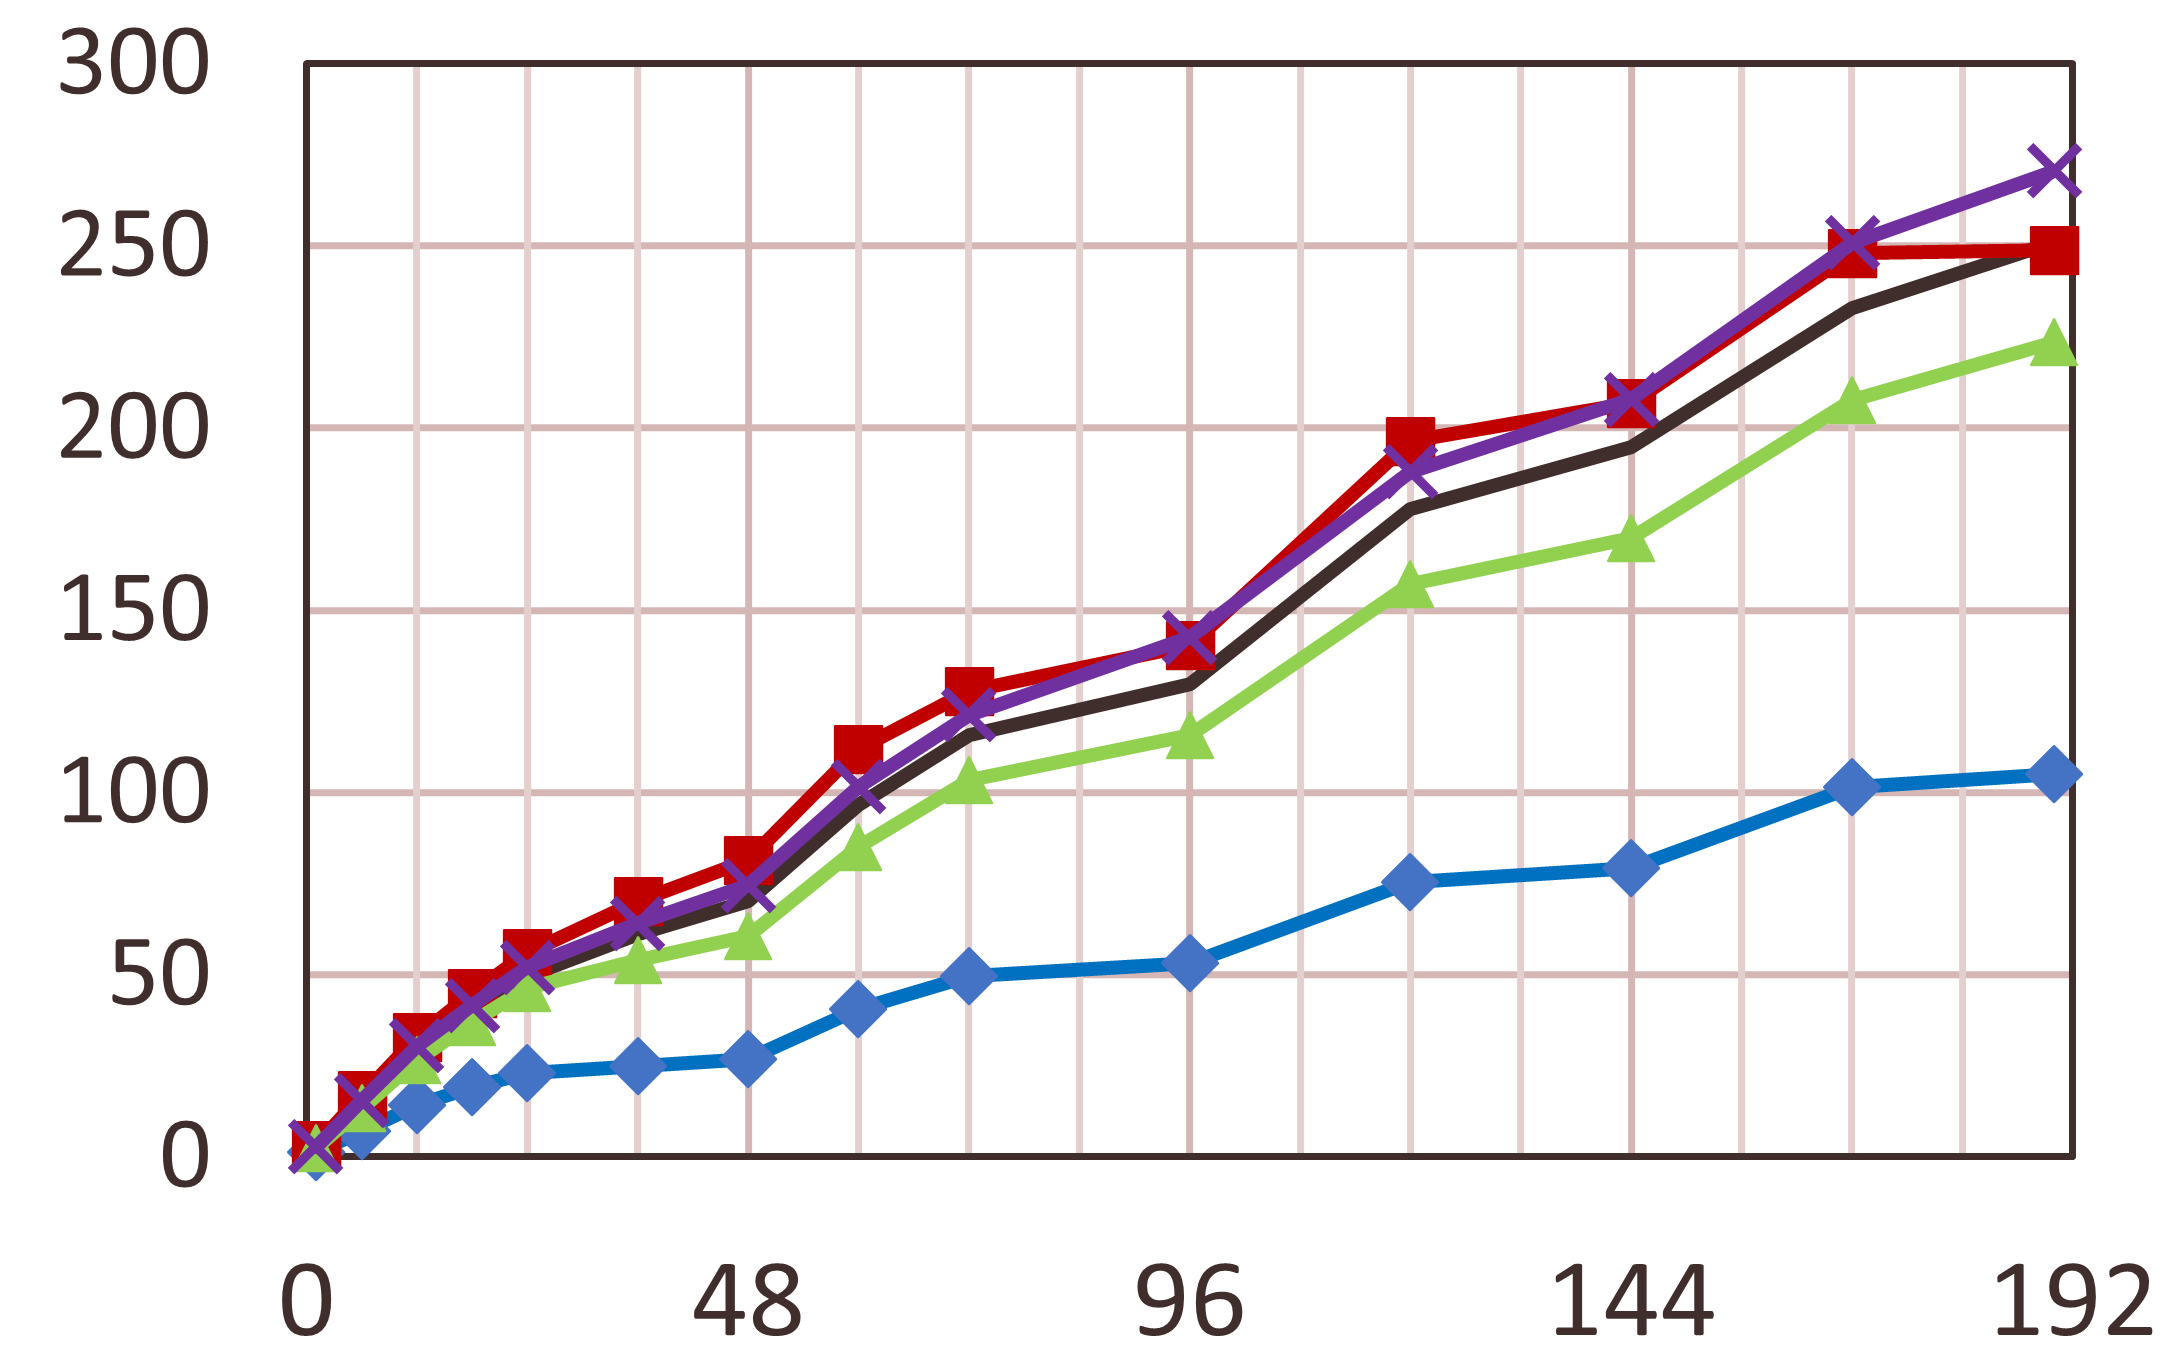
\includegraphics[width=\linewidth]{figures/2021jun16/exp1_nonspec_throughput_exp_'0_0_0_0'_100000_rq_0.png} &
        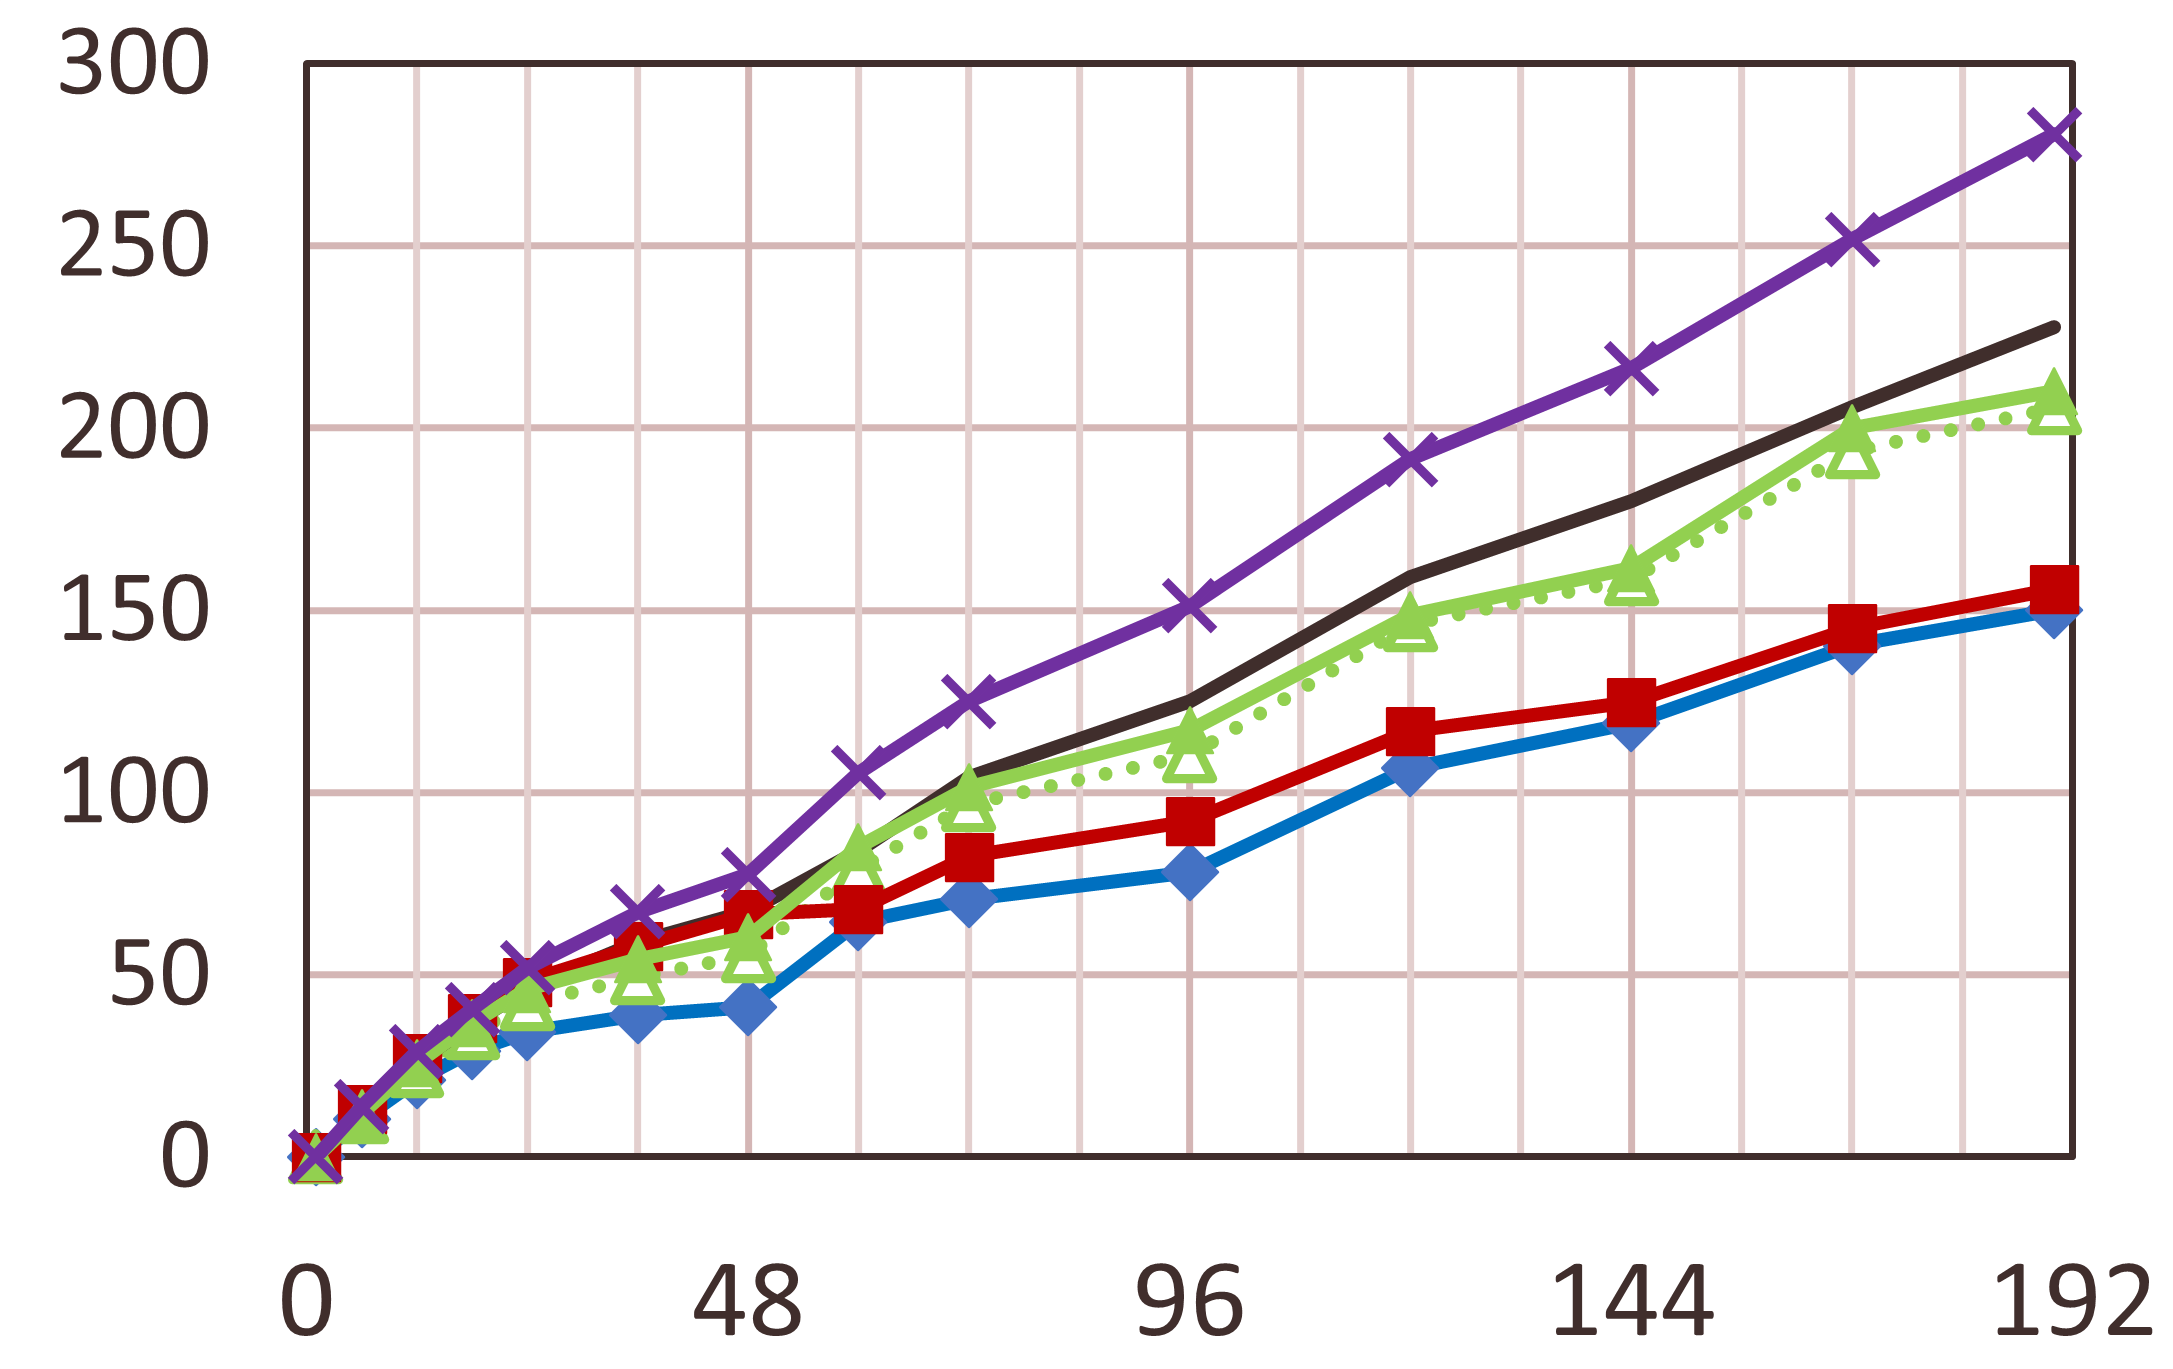
\includegraphics[width=\linewidth]{figures/2021jun16/exp1_nonspec_throughput_exp_'0_0_0_0'_100000_rq_1.png}
        \\
        \vspace{-5mm}\rotatebox{90}{\large 10\% updates} &
        \vspace{-5mm}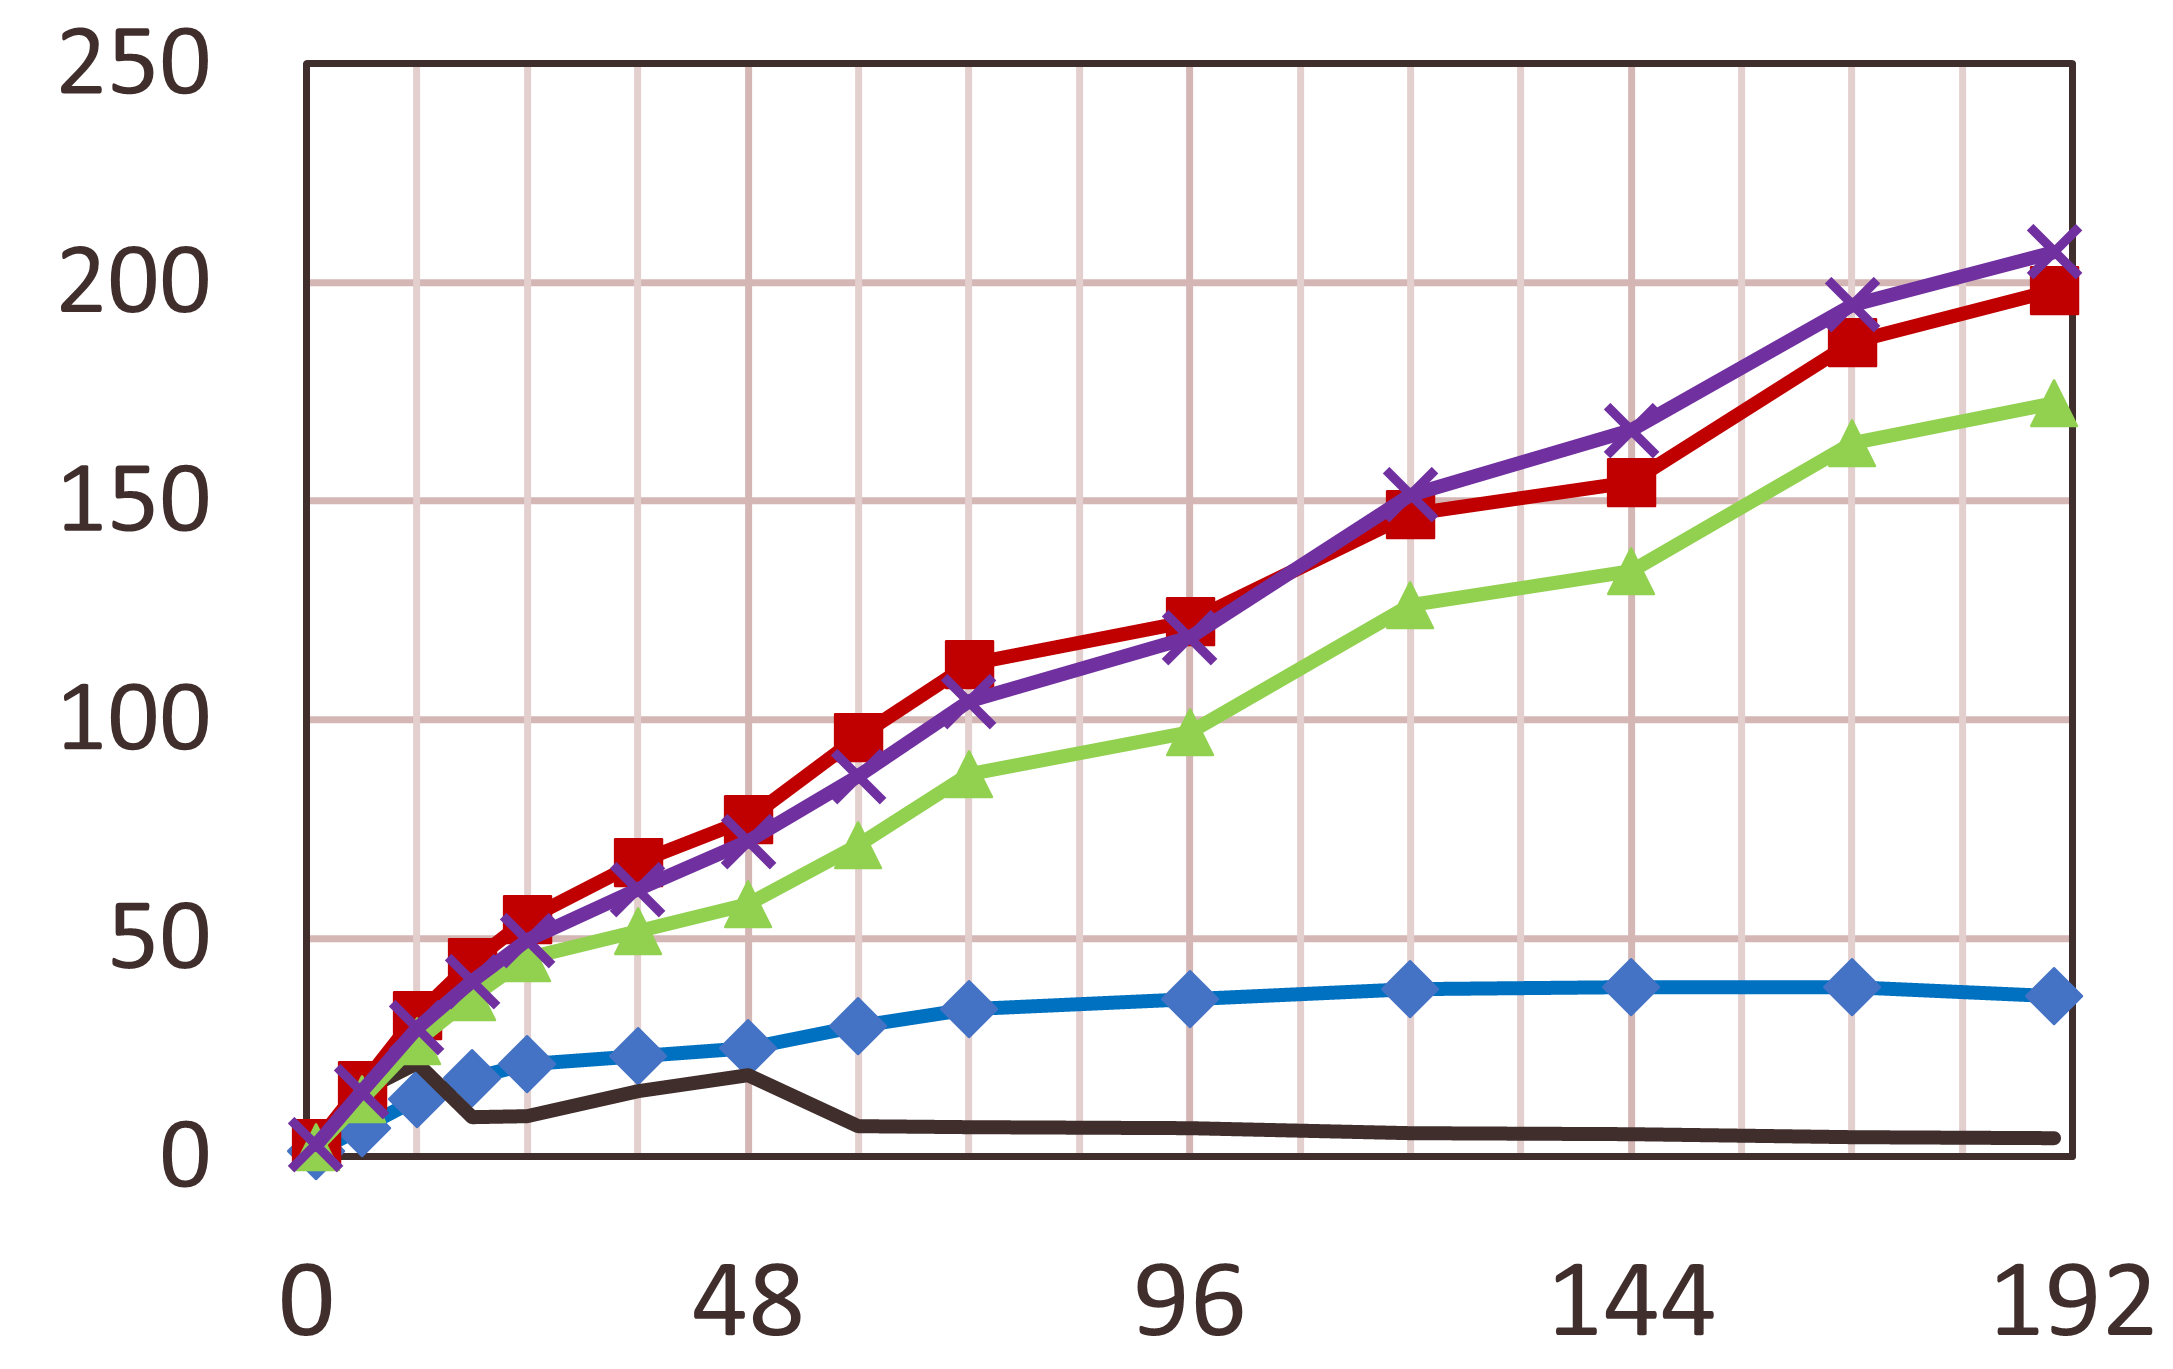
\includegraphics[width=\linewidth]{figures/2021jun16/exp1_nonspec_throughput_exp_'5_0_5_0'_100000_rq_0.png} &
        \vspace{-5mm}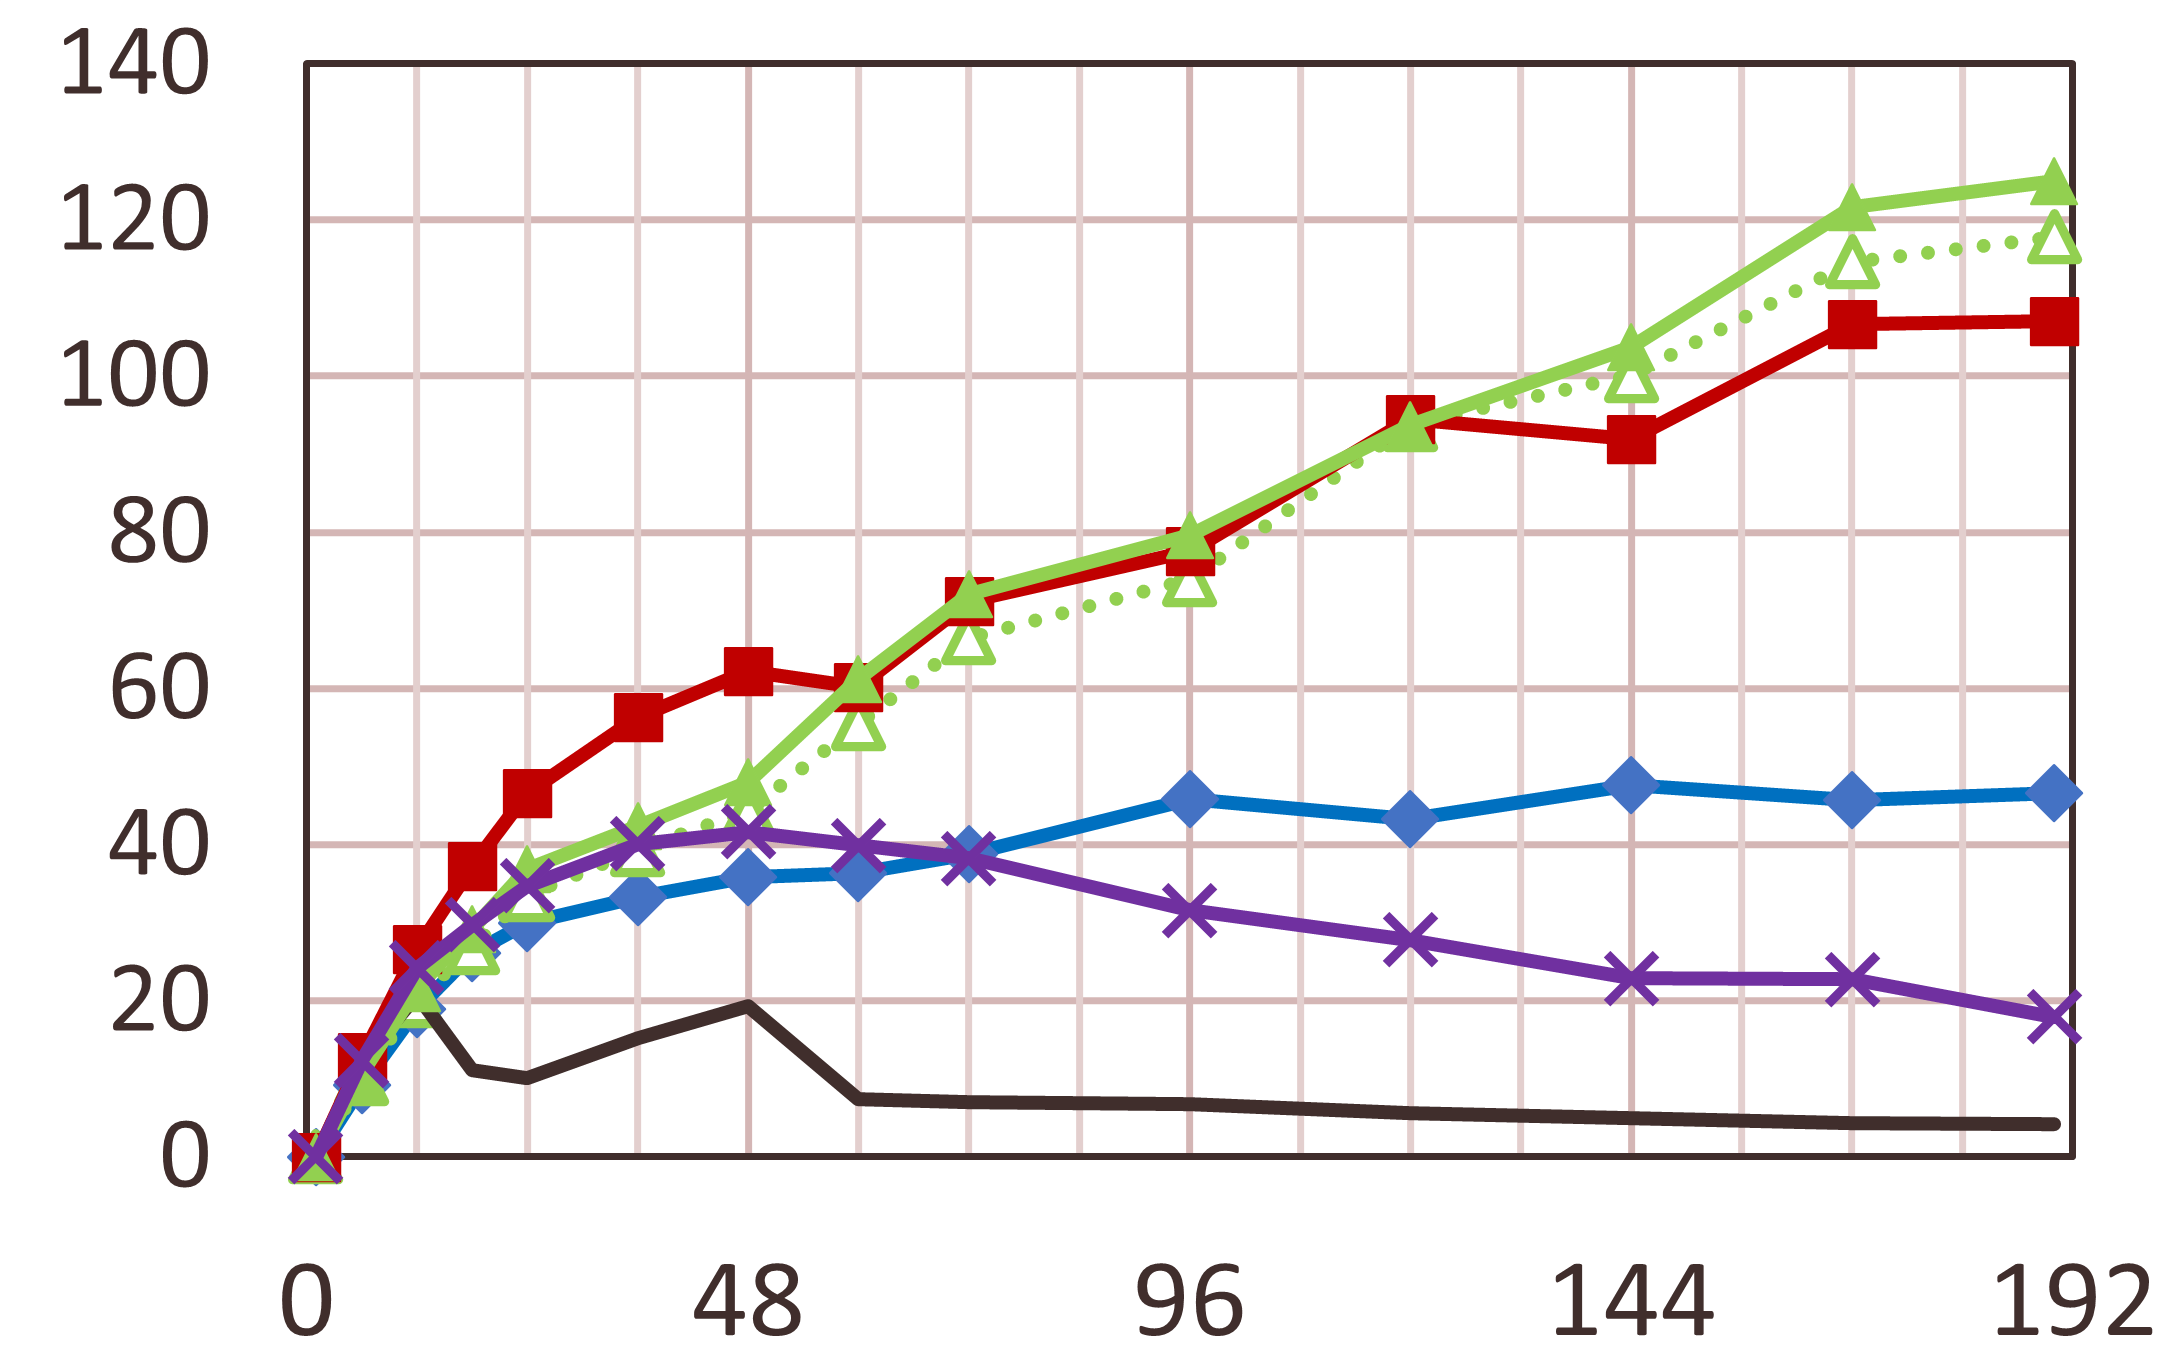
\includegraphics[width=\linewidth]{figures/2021jun16/exp1_nonspec_throughput_exp_'5_0_5_0'_100000_rq_1.png}
        \\
        \vspace{-5mm}\rotatebox{90}{\large 40\% updates} &
        \vspace{-5mm}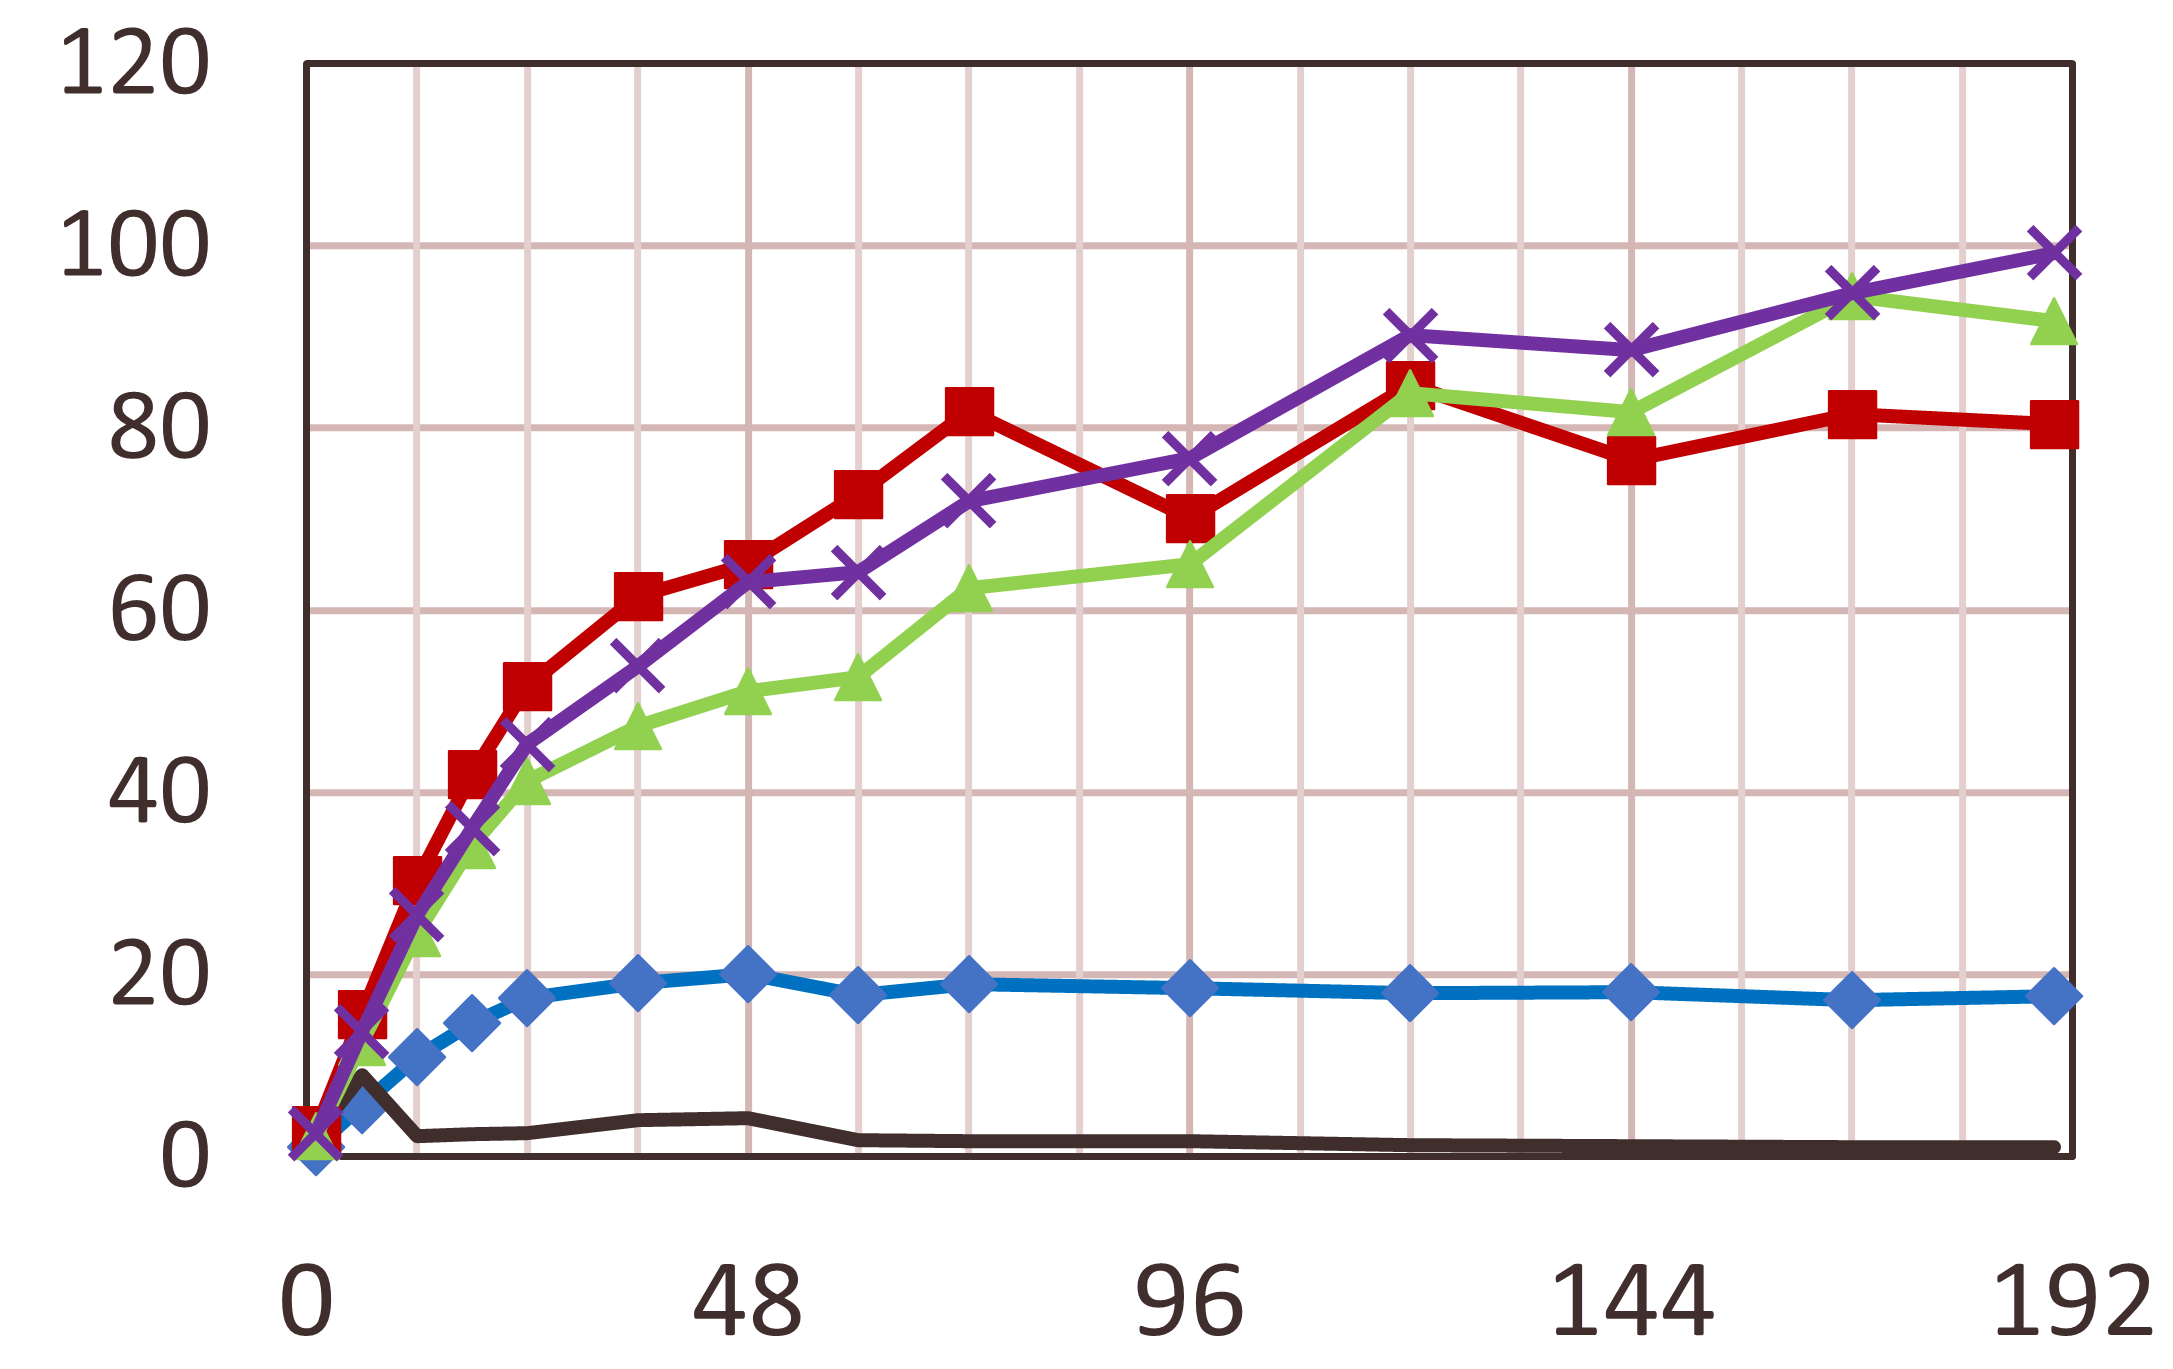
\includegraphics[width=\linewidth]{figures/2021jun16/exp1_nonspec_throughput_exp_'20_0_20_0'_100000_rq_0.png} &
        \vspace{-5mm}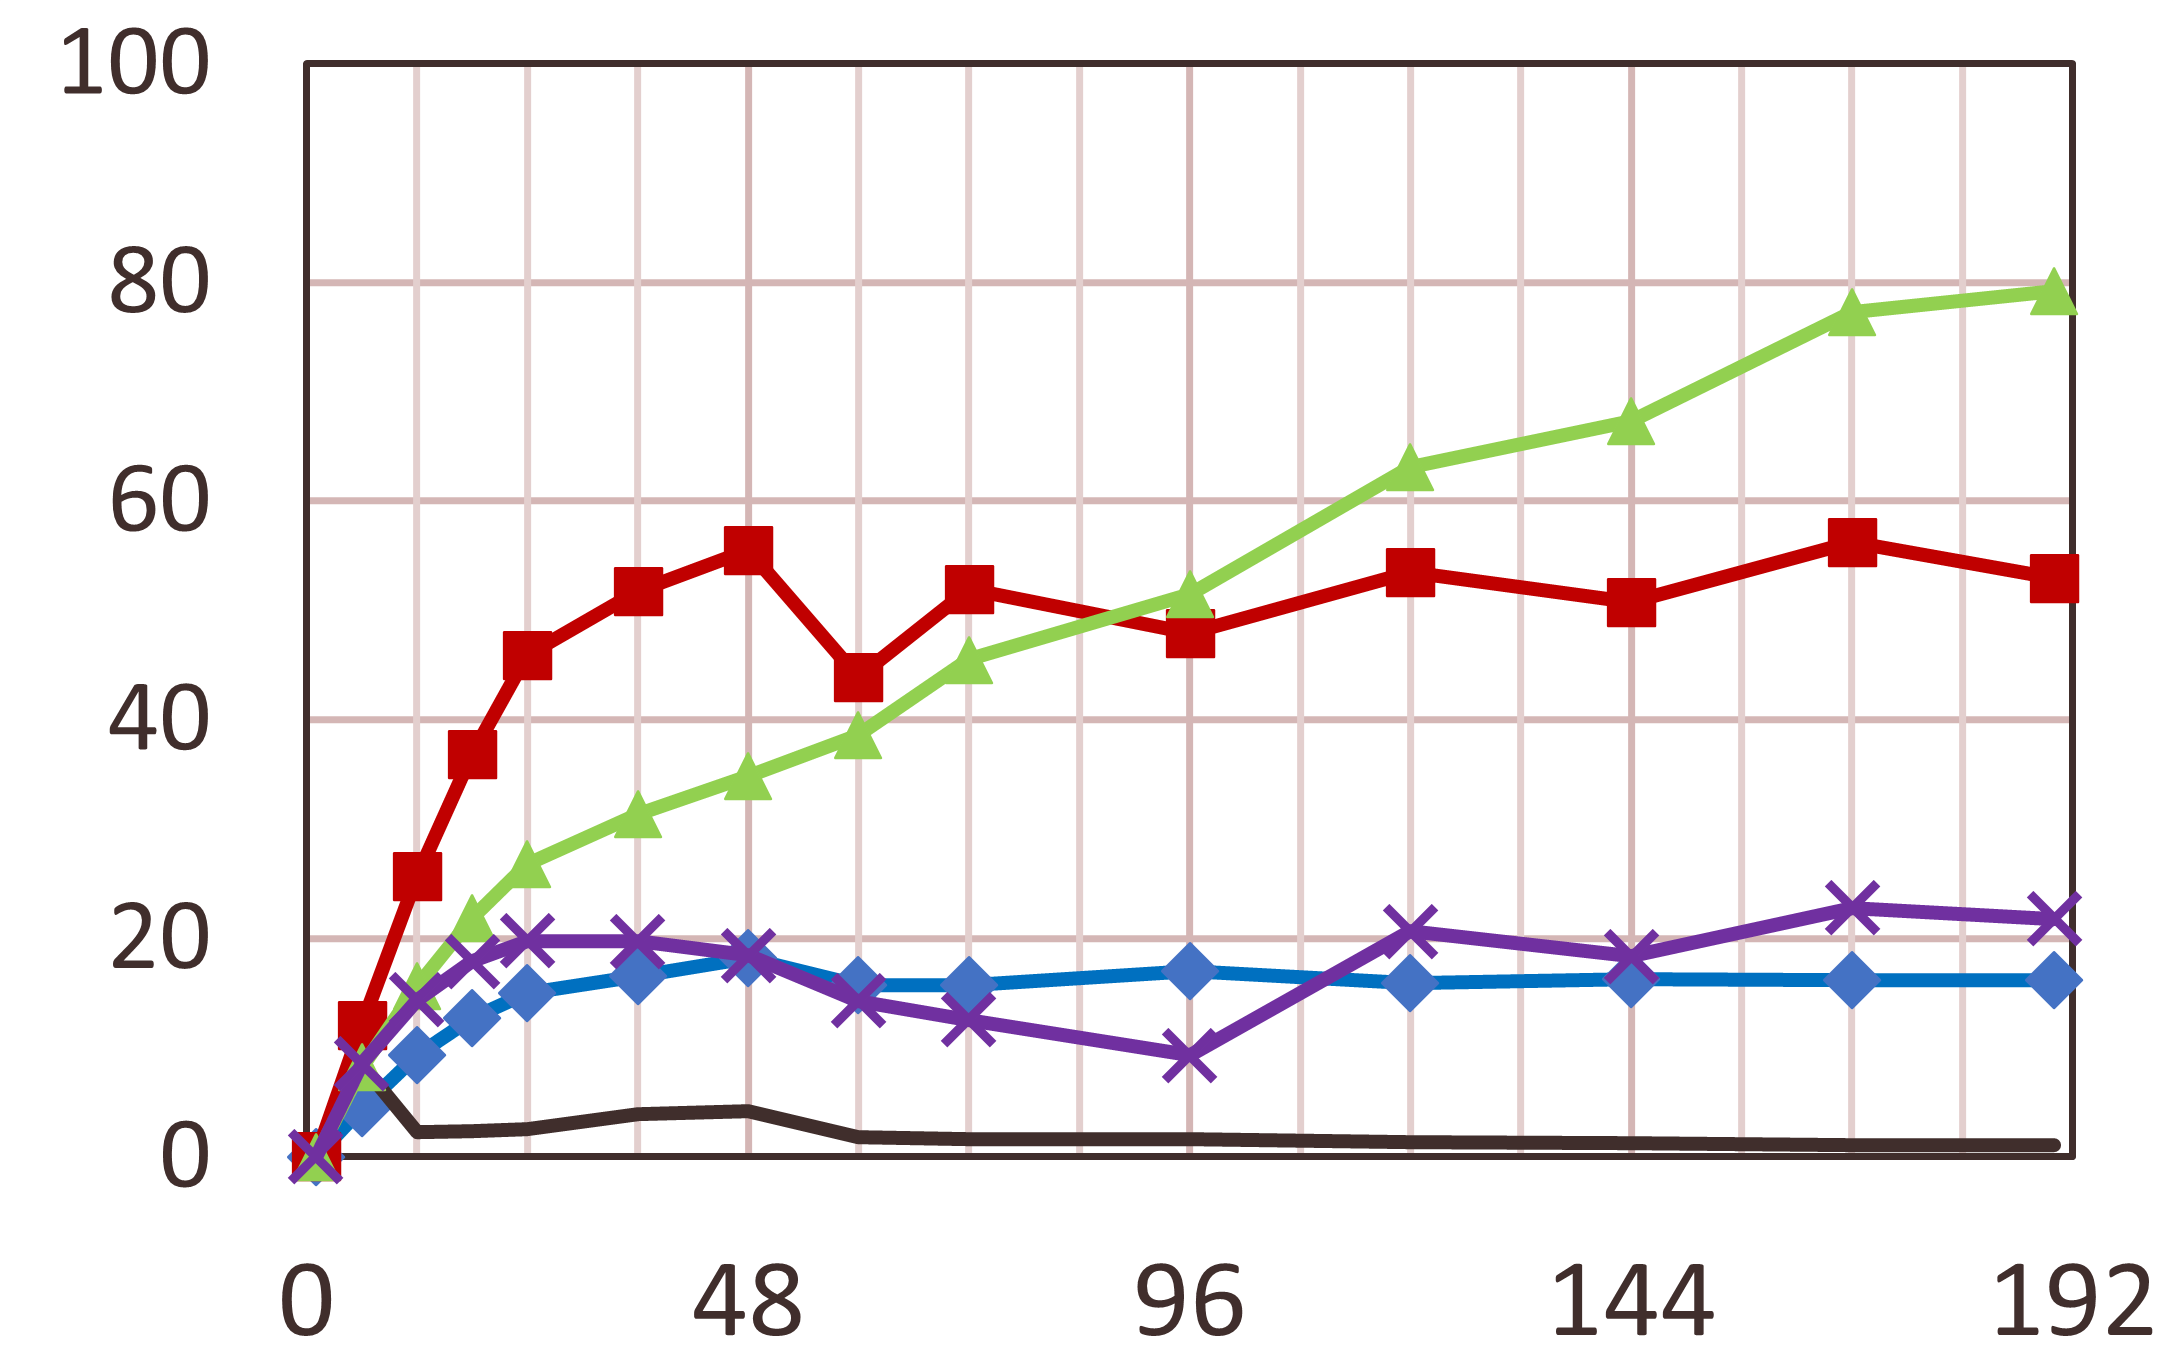
\includegraphics[width=\linewidth]{figures/2021jun16/exp1_nonspec_throughput_exp_'20_0_20_0'_100000_rq_1.png}
        \\
    \end{tabular}
\end{minipage}
%    \vspace{-2mm}
	
\includegraphics[width=.75\linewidth]{figures/2021jun16/legend.png}
%    \vspace{-2mm}
\caption{\textbf{XeonGold} BST benchmark. x-axis: number of threads. y-axis: operations per $\mu$s.}
\label{fig-exp-xeongold}
\end{figure}

\vspace{1mm}\noindent\textbf{Optimizations for this system.}
%
Running on a much larger system with four sockets made it quite evident that some of our implementations were not as scalable as they could be.
So, we further optimized our implementations, obtaining performance improvements primarily from:
\begin{itemize}
\item eliminating several previously undetected instances of false sharing,
\item changing default read/write set sizes (before any dynamic expansion has taken place) from 8192/1024 to 128/64,
\item changing the instrumentation of reads and writes to use branching instead of function pointers to determine which transactional code path to run (fast or fallback), and
\item changing our invocations of \texttt{setjmp} in \textit{TL2} to avoid saving signal masks, which is much more expensive on this large machine.
\end{itemize}

\vspace{1mm}\noindent\textbf{Attempts to port these optimizations to POWER.}
We unfortunately could not run our improved implementations on the POWER8 system because we no longer have access to it.
We attempted to run our code on a newer POWER9 system running FreeBSD, but we discovered that the kernel facilities to expose the necessary HTM capabilities were not implemented on that machine, and although some patches have appeared claiming to add these capabilities, our attempts to apply such patches failed.
We include results from both systems, since we believe they are still instructive, but the following results are not directly comparable with results in the previous subsection.

\vspace{1mm}\noindent\textbf{Dicussion of results.}
See Figure~\ref{fig-exp-xeongold}.
We first discuss the 0\% updates graph for workload type W1.
In this graph, essentially all operations committed in hardware.
In fact, in each trial, a small fraction of 1\% of operations ran on the slow-path.
Thus, any performance differences shown in the graph are essentially differences in the performance of the algorithms' respective fast-paths (with the exception of TL2, which only has one code path).
Algorithm~\ref{alg:inswrite}, which has instrumentation in its fast-path read operations, has significantly lower performance than Algorithm~\ref{alg:inswrite2}, which does not.
Since this is a read-only workload, this instrumentation is responsible for the performance difference.

In W1 workloads with updates, Algorithm~\ref{alg:inswrite2} and Algorithm~1+ perform the best, followed by TLE, then Algorithm~\ref{alg:inswrite}, then TL2 and finally HyNoREC.
In the first three of these algorithms, the fastest code paths have similar amounts of instrumentation: there is no instrumentation for reads or writes, and the transaction itself incurs one or two metadata accesses.
HyNoREC performs very poorly at high thread counts due to its global bottleneck on updates (which affect performance much more when threads run on multiple sockets because of last level cache invalidations).
TL2 suffers mainly due to its high overhead for locking, manipulating explicit read/write sets, and validation costs after each read and at commit time.
Similarly, but to a lesser degree, Algorithm~\ref{alg:inswrite}'s fine-grained instrumentation causes it to lag behind the faster algorithms.

%In the W1 workloads, TLE, Algorithm~\ref{alg:inswrite2} and Hybrid NOrec perform similarly (with a small performance advantage for Hybrid NOrec at high thread counts).
%This is because the fast paths for these three algorithms have similar amounts of instrumentation: there is no instrumentation for reads or writes, 
%and the transaction itself incurs one or two metadata accesses.
In the W2 workloads, the performance of TLE is sometimes spectacularly good (e.g., in W2 with 40\% updates, up to 48 threads), and is other times lackluster (e.g., W2 with 0\% updates, above 48 threads).
%In contrast, in the W2 workloads, TLE performs quite poorly, compared to the HyTM algorithms.
In these workloads, transactions must periodically run on the slow-path, and in TLE, 
this entails acquiring a global lock that restricts progress for all other threads.
When threads run on multiple sockets, this can significantly impact performance.
%We only show Its performance decreases as the sizes of the ranges passed to \textit{RangeIncrement} increase.
%Its performance is also negatively impacted by NUMA effects at thread counts higher than 24.
(This is because, when a thread $p$ reads the lock and incurs a cache miss, 
if the lock was last held by another thread on the same socket, 
then $p$ can fill the cache miss by loading it from the shared L3 cache.
However, if the lock was last held by a thread on a different socket, 
then $p$ must read the lock state from main memory, which is significantly more expensive.)
%On the other hand, in each graph in the W2 workloads, the performance of each HyTM (and TL2) is similar to its performance in the corresponding W1 workload graph.
Similarly, in Algorithm~\ref{alg:inswrite2}, at high thread counts the global commit lock becomes a bottleneck.
The other algorithms all exhibit similar behaviour in W2 graphs to their behaviour in the corresponding W1 graphs.
%
%Although Algorithm~\ref{alg:inswrite2} is not truly progressive, fast-path transactions will abort only if they are concurrent with the commit procedure of a slow-path transaction.
%In \textit{RangeIncrement} operations, there is a long read-only prefix (which is exceptionally long because of Algorithm~\ref{alg:inswrite2}'s quadratic validation) followed by a relatively small set of writes.
%Thus, \textit{RangeIncrement} operations have relatively little impact on the fast-path.
%The explanation is similar for Hybrid NOrec (except that it performs less validation than Algorithm~\ref{alg:inswrite2}).

%Observe that the performance of Hybrid NOrec decreases slightly, relative to Algorithm~\ref{alg:inswrite2}, after 24 threads.
%Recall that, in Hybrid NOrec, the global sequence number is a single point of contention on the fast-path.
%(In Algorithm~\ref{alg:inswrite2}, the global lock is only modified by slow-path transactions, so fast-path transactions do not have a single point of contention.)
%We believe this is due to NUMA effects, similar to those described in~\cite{BKLL16}.
%Specifically, whenever a threads on the first socket performs a fast-path transaction that commits and modifies the global lock, it causes cache invalidations for all other threads.
%Threads on socket two must then load the lock state from main memory, which takes much longer than loading it from the shared L3 cache.
%This lengthens the transaction's window of contention, making it more likely to abort.
%(Inn the 0\% updates graph in the W2 workload, we still see this effect, because there is a thread performing \textit{RangeIncrement} operations.)

Interestingly, the addition of a third code path in Algorithm~1+ allows it to avoid most of the instrumentation overhead of Algorithm~\ref{alg:inswrite} in W1 workloads, while maintaining performance that rivals Algorithm~\ref{alg:inswrite} in more challenging W2 workloads.
In contrast, although Algorithm~\ref{alg:inswrite2} is extremely fast in W1 workloads (and in W2 with 0\% updates), it performs very poorly at high thread counts in W2 with updates.
This suggests that Algorithm~1+ is a better choice for obtaining consistently good performance over a wider variety of workloads.

